\documentclass[10pt,a4paper]{article}

\usepackage[T1]{fontenc}
\usepackage[utf8]{inputenc}
\usepackage{lmodern}
\usepackage[margin=2.2cm]{geometry}
\usepackage{amsmath}
\usepackage{xcolor}
\usepackage{listings}
\usepackage{booktabs}
\usepackage{xltabular}
% A table that never breaks across pages: tabularx in a minipage, with space around it.
\newenvironment{ktab}[2]{\par\medskip\noindent\minipage{\linewidth}\tabularx{#1}{#2}}{\endtabularx\endminipage\par\medskip}
\usepackage{array}
\usepackage{enumitem}
\usepackage[hidelinks,bookmarksnumbered,bookmarksopen]{hyperref}
\usepackage{titlesec}
\usepackage{tikz}

\definecolor{sigbg}{HTML}{F2F4F7}
\definecolor{sigrule}{HTML}{3B6EA5}
\definecolor{codebg}{HTML}{FAFAFA}
\definecolor{kw}{HTML}{1F4E8C}
\definecolor{cm}{HTML}{6A737D}

% A function entry: the signature, then what it does, \params, \returns, and an example last.
\lstdefinestyle{sig}{language=C++, basicstyle=\ttfamily\small\bfseries, backgroundcolor=\color{sigbg},
  frame=leftline, rulecolor=\color{sigrule}, framerule=2pt, xleftmargin=6pt, framexleftmargin=6pt,
  aboveskip=18pt, belowskip=3pt, columns=fullflexible, keepspaces=true, breaklines=false, showstringspaces=false,
  keywordstyle=\color{kw}, morekeywords={Vec2,Vec3,VectorXd,GateState,Domain,Domain2D,ScalarTransport,TransportScheme}}
\lstdefinestyle{ex}{language=C++, basicstyle=\ttfamily\footnotesize, backgroundcolor=\color{codebg},
  frame=single, rulecolor=\color{black!15}, xleftmargin=4pt, framexleftmargin=4pt, aboveskip=4pt,
  belowskip=6pt, columns=fullflexible, keepspaces=true, breaklines=true, keywordstyle=\color{kw},
  commentstyle=\color{cm}, showstringspaces=false}

\usepackage[htt]{hyphenat}
\newcommand{\code}[1]{\texttt{\detokenize{#1}}}
\newenvironment{params}{\par\noindent\textbf{Parameters}\begin{itemize}[leftmargin=1.4em,itemsep=0pt,topsep=1pt,parsep=0pt]}{\end{itemize}}
\newcommand{\p}[2]{\item \code{#1} -- #2}
\newcommand{\returns}[1]{\par\noindent\textbf{Returns}\quad #1\par}
\newcommand{\example}{\par\smallskip\noindent\textbf{Example}\par}

\titleformat{\subsubsection}{\normalfont\bfseries}{\thesubsubsection}{0.8em}{}
\setlength{\parindent}{0pt}
\setlength{\parskip}{3pt}

\title{\textbf{NEREUS 1.0}\\[4pt]\large API Reference}
\author{}
\date{Version 1.0, October 2026}

\begin{document}
\maketitle
\tableofcontents
\newpage

% =====================================================================================================
\section{Introduction}

NEREUS solves the incompressible Navier--Stokes equations in two and three dimensions. It ships three families
of methods. ADI is an Eulerian method with alternating-direction implicit momentum sweeps. FLIP is a hybrid
particle--grid method. SPH is a Lagrangian particle method. The pressure Poisson system is solved on the CPU with
Eigen or AMGCL, or on an NVIDIA GPU with AMGX.

This document describes the classes and functions that a method author or a program uses. It does not describe the
internals of the user interface or of \code{Utils.h}. These are closed boxes.

\subsection{Architecture}

\begin{description}[leftmargin=1em,style=nextline,itemsep=2pt]
\item[The run state is global.] \code{SIMULATION} (\code{Definitions.h}) holds the configuration, the two grids, the
  particle set, the telemetry and the export settings. \code{GRID_ANT} is the field at the start of a step.
  \code{GRID_SOL} is the field the step builds. A solver reads the settings it needs from \code{SIMULATION}. It works
  only on the grids and particles it is handed.
\item[A method is a registered row.] Each method registers one \code{SimulationMethod} row. The row gives the
  method's family, capabilities, settings and initialiser. The library itself names no method. The program
  registers the methods it wants, and the config's \code{TYPE} picks one.
\item[A step is a registered function.] The method's initialiser registers its step functions in order. The shared
  pressure solver registers its own two steps, the pressure solve and the projection. The method only asks for it.
  \code{SimulationManager::StepSimulation} runs the steps. Then it does the work that no solver owns. It computes the
  residual and the telemetry, copies the grid, writes the exports, checks the stopping rule and saves checkpoints.
\item[The grid is \code{MAC}, a staggered marker-and-cell grid, uniform or stretched.] The velocity lives on the cell
  faces. The pressure and any registered scalars live at the cell centres. Every cell has a type, and the grid holds
  the spacing tables and the boundary conditions as recorded index lists.
\end{description}

\subsection{Conventions}

\begin{itemize}[itemsep=1pt]
\item \textbf{Index order.} Every accessor takes \code{(i, j, k)}. Here \code{i} is the row (y), \code{j} is the
  column (x) and \code{k} is the layer (z). The 2D overloads take \code{(i, j)}. All fields are stored in this order.
\item \textbf{Staggering.} \code{u} sits on the x faces, \code{v} on the y faces and \code{w} on the z faces.
  \code{p} and the scalars sit at the cell centres. A velocity component has one more entry along its own axis, so
  \code{u} has $(N_x{+}1)\times N_y\times N_z$ entries and \code{p} has $N_x\times N_y\times N_z$. Face \code{j} of
  \code{u} lies between cells \code{j-1} and \code{j}.
\item \textbf{Components and axes} are the enums \code{MAC::Component} (\code{U}, \code{V}, \code{W}, \code{P}) and
  \code{MAC::Axis} (\code{X}, \code{Y}, \code{Z}), written \code{MAC::U} or \code{MAC::X}.
\item \textbf{Cell types.} \code{FLUID_CELL} (0), \code{SOLID_CELL} (1), \code{EMPTY_CELL} (2), \code{INFLOW_CELL}
  (3), \code{PRESSURE_CELL} (4) and \code{OUTFLOW_CELL} (5). A cell type says what the solvers do with a cell.
  \code{SOLID_CELL} is a wall or an obstacle. \code{EMPTY_CELL} is air in FLIP, and a pressure outlet at zero pressure
  on the ring. \code{PRESSURE_CELL} is a pressure outlet with a given pressure. \code{INFLOW_CELL} is an inlet and
  \code{OUTFLOW_CELL} a continuity outflow.
\item \textbf{The ring.} The grid has one extra layer of cells outside the domain on every side, the \emph{ring}. It
  carries the boundary conditions. So the walls lie exactly on the faces of the domain, and \code{GRID_SIZE} counts
  only the cells inside the domain.
\item \textbf{Coordinates} are physical, in metres, read from the spacing tables.
\item \textbf{Units} are SI throughout:
\end{itemize}
\begin{ktab}{\linewidth}{@{}>{\raggedright}p{0.36\linewidth} >{\raggedright}p{0.18\linewidth} X@{}}
\toprule
\textbf{Quantity} & \textbf{Unit} & \textbf{Note} \\
\midrule
lengths, coordinates, \code{dh} & m & \\
time, \code{dt}, \code{t} & s & \\
velocity & m/s & \\
pressure & Pa & the real pressure, not divided by the density \\
density \code{DENSITY} & kg/m$^3$ & \\
viscosity \code{VISCOSITY} & m$^2$/s & kinematic \\
body force \code{Fu}, \code{Fv}, \code{Fw}, scene \code{force} & m/s$^2$ & an acceleration, added as $f\,\Delta t$ \\
divergence & 1/s & \\
scalars & any & as the user defines them \\
\bottomrule
\end{ktab}

% =====================================================================================================
\section{Getting Started with a Custom Method}\label{sec:tutorial}

This tutorial builds the program, runs a shipped case, and then writes a complete method. The method is
\code{EXPLICIT}, the smallest one in the code: forward-Euler momentum, its own pressure solve by successive
over-relaxation (SOR), and the projection. It lives in \code{src/Methods/Explicit/}, three files of fewer than two
hundred lines in all, and adding it changed no file of the library. Every listing is the real code. The functions it
calls are described in full in the later sections.

\subsection{Build}

Build with \code{make} from the repository's root. It needs a C++17 compiler: GCC on Linux and on Windows (MSYS2),
Clang on macOS. Eigen and GLFW ship with the repository. OpenMP is used when the compiler has it. The GPU pressure
solver needs AMGX and CUDA, and is built on Linux only, when both are found.

\begin{ktab}{\linewidth}{@{}>{\raggedright}p{0.36\linewidth} X@{}}
\toprule
\textbf{Command} & \textbf{Builds} \\
\midrule
\code{make -j} & \code{bin/nereus}, the program with its window. \\
\midrule
\code{make HEADLESS=1 -j} & \code{bin/nereus_headless}, with no window and no graphical library linked. \\
\midrule
\code{make NVIDIA_GPU=0 -j} & a program with the CPU pressure solvers only. \\
\midrule
\code{make DEBUG=1 -j} & a debug build, with assertions and bounds checks. \\
\midrule
\code{make info} & nothing. It prints what a build would use. \\
\bottomrule
\end{ktab}

\subsection{Run a case}

The folder \code{configs/} holds one file per case, grouped by benchmark. Each file is complete: the method, the
grid, the fluid, the stopping rule, the exports and the scene.

\textbf{With the window.} \code{bin/nereus} opens the setup screen. Pick a case, for example the cavity
\code{Explicit/ldc_2d_re100_explicit}, and press \emph{Start}. The top bar runs, pauses and steps the simulation.

\textbf{Without a window.} The same file runs from the command line.
\begin{lstlisting}[style=ex]
bin/nereus_headless configs/Explicit/ldc_2d_re100_explicit.cfg
bin/nereus --headless configs/Explicit/ldc_2d_re100_explicit.cfg --progress 100
\end{lstlisting}
\begin{ktab}{\linewidth}{@{}>{\raggedright}p{0.30\linewidth} X@{}}
\toprule
\textbf{Option} & \textbf{Meaning} \\
\midrule
\texttt{-{}-headless [\textless{}config\textgreater{}]} & run the config with no window. The GUI program accepts it too. \\
\midrule
\texttt{-{}-progress N} & print a progress line every \code{N} steps (default 100, 0 for none). \\
\midrule
\texttt{-{}-quiet} & print the summary only. \\
\bottomrule
\end{ktab}
The exit code is 0 when the stopping rule ended the run, 1 for a usage error, a config file that does not exist or
is not valid (below), a \code{TYPE} that names no registered method, or a config that nothing would stop, 2
when the field stopped being finite (it is checked after every step), and 3 when the run was interrupted. An
interrupted run writes its checkpoint first.

\textbf{The output.} Every file of a run goes to one folder,
\begin{lstlisting}[style=ex]
<EXPORT_BASE_PATH>/<config name>/<GRID_SIZE>_<2D|3D>_re<REYNOLDS_NUMBER>/
\end{lstlisting}
It holds \code{telemetry.csv}, one row per telemetry interval, and the field frames in \code{VTK/} as
\code{grid-NNNN.vtr} files for ParaView, numbered by frame (the final field, written when the stopping rule fires, is
one more frame). A \code{.vtr} is a rectilinear grid with one point per cell centre, the ring included. It carries
\code{Velocity} (each component the mean of the cell's two faces), \code{Pressure}, \code{Divergence}, \code{Solid}
(the cell type) and one array per registered scalar. The particle methods add particle files and, in 3D, liquid
surfaces.

\subsection{The case file}

A config file has \code{KEY = value} lines, then blocks for the pressure solver, for each method's settings and for
the scene. A key that is left out takes its default (\code{DIMENSION} defaults to 3, so a 2D case must say so). The
reader refuses a file it cannot trust, listing every problem before the run starts: a key no reader knows, at the top
level or inside a method block; a number or an integer that does not parse in full (\code{VISCOSITY = 0.01abc}); a
choice outside its list (\code{CONVECTION_SCHEME = CENTRALL}); a malformed refinement interval; and a block for a
method the program did not register. Section~\ref{sec:config} lists every key, and Section~\ref{sec:telemetry} every
telemetry column. This is the lid-driven cavity at Re 100 the tutorial runs,
\code{configs/Explicit/ldc_2d_re100_explicit.cfg}, shortened.
\begin{lstlisting}[style=ex]
DIMENSION = 2
TYPE = EXPLICIT                 # the key of a registered method
THREAD_COUNT = 1
DOMAIN_X0 = 0
DOMAIN_XF = 1
DOMAIN_Y0 = 0
DOMAIN_YF = 1
GRID_SIZE = 32                  # cells across the shorter side
VISCOSITY = 0.01                # kinematic, m^2/s
DENSITY = 1
TIME_STEP = 0.01                # the largest step; ADAPTATIVE_TIMESTEP only shrinks it
ADAPTATIVE_TIMESTEP = 1
MAX_CFL = 0.5
STOP_CONDITION = TIME           # NEVER, TIME or RESIDUAL
STOP_TIME = 60
EXPORT_ENABLED = 1
EXPORT_GRID = 1
EXPLICIT_BEGIN                  # the method's own block, read through its settings table
EXPLICIT_RELAXATION = 1.7
EXPLICIT_TOLERANCE = 1e-06
EXPLICIT_MAX_ITERATIONS = 10000
EXPLICIT_END
SCENE_BEGIN
boundary xmin noslip
boundary xmax noslip
boundary ymin noslip
boundary ymax moving u="1"   # last, so the lid wins the two top corners
SCENE_END
\end{lstlisting}
The scene gives each face of the domain a boundary kind, here three no-slip walls and a moving lid. Regions add solids
or, for a particle method, the initial liquid. Probes add telemetry columns (Section~\ref{sec:scene-api}). To try
another method on the same case, change \code{TYPE}: \code{TYPE = ADI} runs the same cavity with the ADI method. The
setup screen edits the same file and saves the whole of it back, so a file written by hand and one written on screen
are interchangeable.

\subsection{The program}

A program registers the methods it can run, starts a run from a config file, steps it, and releases the pressure
solver at the end. The library names no method, so a program that leaves a method out is built without it.
\begin{lstlisting}[style=ex]
#include "headers/Core/SimulationManager.h"
#include "Methods/ADI/ADISettings.h"
#include "Methods/Explicit/ExplicitSettings.h"

int main()
{
    RegisterADI();                                   // before any config is read
    RegisterExplicit();
    SimulationManager::InitializeSimulation("configs/Explicit/ldc_2d_re100_explicit.cfg");
    if (SIMULATION.exports.enabled) Exports::InitializeTelemetry();
    SIMULATION.running = true;
    while (SIMULATION.running)                       // false once the stopping rule fires
        SimulationManager::StepSimulation();
    SimulationManager::DisposeSimulation();          // frees the method, the grids and the steps
    return 0;
}
\end{lstlisting}
The registration comes first because the config's \code{TYPE} is looked up in the registry, and building the grid
asks the method whether it allows a stretched grid. \code{Exports::InitializeTelemetry} names the telemetry file and
writes its header; the file opens at the first row. A program without a window calls it only when exports are on,
the window's loop calls it always, since export can be switched on during the run. With a window, the four calls of Section~\ref{sec:ui-api} wrap
the same loop. The shipped \code{src/main.cpp} is this program, with both.

\subsection{A method of your own}

The method is a folder of its own. The Makefile compiles every \code{src/Methods/*/*.cpp}, so the folder needs no
build change, and the program registers the method with one line, \code{RegisterExplicit();}, once it includes the
method's settings header. Every object file is built into one folder and every method is linked into one program, so
a \code{.cpp} file name must be unique across \code{src/}, and the method's classes, namespaces and global names must
not clash with another method's (the explicit method keeps its own inside \code{Explicit2D}).
\begin{lstlisting}[style=ex]
src/Methods/Explicit/
  Explicit2D.h          the declarations of the step functions
  Explicit2D.cpp        momentum, pressure, projection, stable time step
  ExplicitSettings.h    the settings struct and table, InitializeExplicit, RegisterExplicit
\end{lstlisting}

\subsubsection*{Step 1: the settings}

The settings are a plain struct with one global instance, and a table (Section~\ref{sec:settings-api}). From the
table alone the config reader fills the struct from the \code{EXPLICIT} block, and the setup screen draws an input
box for each real number and a slider for the bounded integer.
\begin{lstlisting}[style=ex]
struct ExplicitSettings
{
    double relaxation = 1.7;      // SOR factor: 1 is plain Gauss-Seidel
    double tolerance = 1e-6;      // stop when no cell's equation is off by more than this times the largest source
    int maxIterations = 10000;
};
inline ExplicitSettings EXPLICIT_SETTINGS;

inline const SettingField EXPLICIT_FIELDS[] = {
    DoubleSetting("EXPLICIT_RELAXATION", "SOR relaxation", "SOR over-relaxation factor, 0.5 to 2",
                  offsetof(ExplicitSettings, relaxation), 1.7, 0.5, 2.0),
    DoubleSetting("EXPLICIT_TOLERANCE", "Pressure tolerance", "Largest residual relative to the largest right-hand side",
                  offsetof(ExplicitSettings, tolerance), 1e-6, 1e-14, 1.0),
    IntSetting("EXPLICIT_MAX_ITERATIONS", "Max sweeps", "", offsetof(ExplicitSettings, maxIterations), 10000, 1, 1e7),
};
\end{lstlisting}

\subsubsection*{Step 2: the row}

The row is everything the rest of the code knows about the method (Section~\ref{sec:registry}).
\begin{lstlisting}[style=ex]
static inline void RegisterExplicit()
{
    RegisterSimulationMethod({"EXPLICIT", "Explicit (Eulerian)",
        "Forward Euler momentum and an SOR pressure solve, 2D uniform grids",
        MethodFamily::EULERIAN, true, false, CAP_GRID | CAP_BOUNDARY_CELLS | CAP_FIXED_REGION,
        InitializeExplicit, nullptr,
        &EXPLICIT_SETTINGS, EXPLICIT_FIELDS, (int)(sizeof(EXPLICIT_FIELDS) / sizeof(EXPLICIT_FIELDS[0])), nullptr,
        nullptr, Explicit2D::StableTimestep, nullptr, nullptr, nullptr});
}
\end{lstlisting}
The row runs in 2D only. It leaves three capabilities off on purpose: without \code{CAP_RECTILINEAR} it is given a
uniform grid, without \code{CAP_SCALARS} no scalars are transported, and without \code{CAP_PRESSURE_SOLVER} the setup
screen does not show the shared pressure solver's settings. \code{stableTimestep} gives the method's own stability
limit (Step~6). The other questions are null, so the manager answers them from the grid.

\subsubsection*{Step 3: the steps}

The initialiser seeds the grids from the scene and registers three step functions (Section~\ref{sec:steps-api}). The
manager runs them in order every time step and times each one.
\begin{lstlisting}[style=ex]
static inline void InitializeExplicit()
{
    MAC::InitializeSimulationGrids();
    RegisterSimulationStep(Explicit2D::Momentum, "momentum", 0);
    RegisterSimulationStep(Explicit2D::Pressure, "pressure", 4);
    RegisterSimulationStep(Explicit2D::Projection, "projection", 6);
}
\end{lstlisting}
\code{MAC::InitializeSimulationGrids} (Section~\ref{sec:mac-construction}) seeds both of the run's grids from the
scene and gives each the boundary functions.

\subsubsection*{Step 4: momentum}

On every face between two fluid cells,
\begin{equation*}
  \mathbf u^* = \mathbf u^n + \Delta t\,\bigl(-(\mathbf u^n\cdot\nabla)\mathbf u^n + \nu\nabla^2\mathbf u^n
   + \mathbf f\bigr),
\end{equation*}
with central differences. The Laplacian of a face value $u$ sums over its four neighbours $u_m$,
\begin{equation*}
  \nabla^2 u \approx \frac{1}{h^2}\sum_{m} f_m\,(u_m - u),
\end{equation*}
where $f_m$ is the wall factor of Section~\ref{sec:mac-bc}. It is the ratio between the distance the stencil assumes,
one cell, and the true distance to where the neighbour's value belongs.
\begin{itemize}[itemsep=1pt,topsep=2pt]
\item \textbf{A face in the middle of the domain.} Its neighbour $u_m$ is another face one cell away, where its
  value is stored. The distance is right, so $f_m = 1$.
\item \textbf{A face in the first row beside a no-slip wall.} The neighbour across the wall is the ring value, which
  holds the wall velocity $u_w$. That value belongs on the wall, the boundary face, which is only half a cell away. The
  difference $u_w - u$ must be divided by $h/2$, not $h$, so $f_m = 2$: the term $2(u_w - u)$ is the same as a ghost
  value $2u_w - u$ reflected through the wall, one cell away.
\end{itemize}
A slip wall, an inlet or an outlet has its value where the stencil expects it, so $f_m = 1$ there too. The function
\code{MAC::WallLinkFactor} returns $f_m$ for every coupling, so the loop needs no special case for walls. The convection is
written in the advective form, $(\mathbf u\cdot\nabla)\mathbf u$, which keeps a uniform field uniform but does not
conserve momentum or kinetic energy discretely. Its central difference next to a wall reads the ring value as if it
were a full cell away; this simple method does not correct that, which leaves the convective term first order in the
first row beside a wall.
\begin{lstlisting}[style=ex]
static double Laplacian(MAC *g, MAC::Component c, int i, int j)
{
    const double u = g->GetComponent(c, i, j);
    double sum = 0.0;
    for (int s = -1; s <= 1; s += 2)
        sum += g->WallLinkFactor(c, MAC::X, i, j, s) * (g->GetComponent(c, i, j + s) - u)
             + g->WallLinkFactor(c, MAC::Y, i, j, s) * (g->GetComponent(c, i + s, j) - u);
    return sum / (g->dh * g->dh);
}

void Explicit2D::Momentum(MAC *ant, MAC *sol, ParticleSet *, double time)
{
    const double dt = SIMULATION.dt, nu = SIMULATION.EPS, h2 = 2.0 * ant->dh;
    sol->CopyFlowFields(*ant);
    for (int i = 1; i < ant->Ny - 1; i++)
        for (int j = 1; j < ant->Nx; j++)
            if (ant->FaceGate(MAC::U, i, j) == GateState::OPEN)
            {
                const double u = ant->GetU(i, j), v = ant->getVatU(i, j);
                const double dudx = (ant->GetU(i, j + 1) - ant->GetU(i, j - 1)) / h2;
                const double dudy = (ant->GetU(i + 1, j) - ant->GetU(i - 1, j)) / h2;
                sol->SetU(i, j, u + dt * (-u * dudx - v * dudy + nu * Laplacian(ant, MAC::U, i, j)));
            }
    /* ... the same loop for v ... */
    sol->AddForce(time, dt);
    sol->EnforceVelocityBC(time + dt);
}
\end{lstlisting}
The step leaves the faces next to the ring alone. \code{EnforceVelocityBC} sets them for every boundary kind, whether
wall, inlet or outlet, so the method runs any scene the code can describe, obstacles included.

\subsubsection*{Step 5: pressure and projection}

The pressure solves
\begin{equation*}
  \nabla^2 p = \frac{\rho}{\Delta t}\,\nabla\cdot\mathbf u^*
\end{equation*}
on the fluid cells. For a cell with pressure $p$ and right-hand side $b$, scaled by $h^2$, the discrete equation is
\begin{equation*}
  \sum_{n} c_n\,(p_n - p) = b, \qquad
  c_n = \begin{cases} 1 & \text{neighbour fluid (an unknown)},\\
                      2 & \text{neighbour a pressure-outlet ring cell (a known value half a cell away)},\\
                      0 & \text{neighbour a wall or an inlet (known velocity: no flux)}.\end{cases}
\end{equation*}
With $D = \sum_n c_n$, the residual of the cell and the SOR update are
\begin{equation*}
  r = \sum_n c_n\,p_n - D\,p - b, \qquad p \leftarrow p + \omega\,\frac{r}{D}.
\end{equation*}
For $\omega = 1$ this is Gauss--Seidel: $r/D$ is the change that satisfies the cell's equation. The relaxation
$\omega$ is \code{EXPLICIT_RELAXATION}.

\noindent\begin{minipage}{\linewidth}
\begin{lstlisting}[style=ex]
double sum = 0.0, diag = 0.0;
for (int n = 0; n < 4; n++)
{
    const int ni = i + di[n], nj = j + dj[n];
    const bool outlet = g->IsPressureOutlet(ni, nj);
    const double c = g->IsFluid(ni, nj) ? 1.0 : (outlet ? 2.0 : 0.0);
    sum += c * g->GetP(ni, nj);
    diag += c;
}
const double p = g->GetP(i, j);
const double r = sum - diag * p - b[i * nx + j];   // how far the equation is from being satisfied
g->SetP(i, j, p + w * r / diag);                  // r / diag zeroes it; w over-relaxes
\end{lstlisting}
\end{minipage}

\code{IsFluid} and \code{IsPressureOutlet} are the grid's cell queries (Section~\ref{sec:mac}); the second is true
for the two ring types of a pressure outlet, \code{EMPTY_CELL} and \code{PRESSURE_CELL}. The sweeps stop when the
largest $|r|$ is below \code{EXPLICIT_TOLERANCE} times the largest $|b|$, or after \code{EXPLICIT_MAX_ITERATIONS}
sweeps. A method that brings its own solver also decides what to do and report when it does not converge; the
explicit method stops silently. With no outlet the pressure is fixed only up to a constant, and its mean is set to
zero afterwards.
\code{EnforcePressureBC} runs before the sweeps, for the outlet values, and after them, so each wall ring cell copies
its neighbour.

The projection then corrects every face that is not a wall,
\begin{equation*}
  \mathbf u^{n+1} = \mathbf u^* - \frac{\Delta t}{\rho}\,\nabla p,
\end{equation*}
with the gradient taken over the half cell on a face beside an outlet ring cell.
\begin{lstlisting}[style=ex]
if (g->FaceGate(MAC::U, i, j) != GateState::WALL)
{
    const bool half = g->IsPressureOutlet(i, j) || g->IsPressureOutlet(i, j - 1);
    g->SetU(i, j, g->GetU(i, j) - (half ? 2.0 : 1.0) * k * (g->GetP(i, j) - g->GetP(i, j - 1)));
}
\end{lstlisting}

\subsubsection*{Step 6: the stable time step}

Forward Euler with central differences, in 2D, is stable when the step is below the two limits
\begin{equation*}
  \Delta t \le \frac{h^2}{4\nu}, \qquad \Delta t \le \frac{2\nu}{|u|^2},
\end{equation*}
the diffusive limit and the convective one of a central scheme. Together they imply the CFL condition
$\Delta t \le h/|u|$, which the code also checks, as a guard on how far the flow moves in one step. The row's
\code{stableTimestep} returns the smallest of the three times \code{MAX_CFL}. The manager uses it under
\code{ADAPTATIVE_TIMESTEP}. Without that key \code{TIME_STEP} is used as given, and nothing checks it.
\begin{lstlisting}[style=ex]
double Explicit2D::StableTimestep()
{
    const double h = SIMULATION.GRID_ANT->dh, nu = SIMULATION.EPS;
    const double u = std::max(SIMULATION.GRID_ANT->GetMaxVelocity(), 1e-6);
    return MAX_CFL * std::min({h / u, h * h / (4.0 * nu), 2.0 * nu / (u * u)});
}
\end{lstlisting}

\subsubsection*{Step 7: run it}

Build, then run the case of the tutorial.
\begin{lstlisting}[style=ex]
make HEADLESS=1 -j
bin/nereus_headless configs/Explicit/ldc_2d_re100_explicit.cfg
\end{lstlisting}
Every step the manager runs \code{momentum}, \code{pressure} and \code{projection}, then the residual, the
telemetry and the exports (Section~\ref{sec:manager}). At $t = 60$ the stopping rule fires and writes the final field
to \code{VTK/}. The telemetry has one \code{<name>_timing} column per step, so the method is profiled with no code of
its own.

\subsubsection*{Possibilities for extension}

\begin{itemize}[itemsep=1pt]
\item Add an obstacle: \code{region solid cylinder axis=z center=(0.5,0.5) radius=0.1} in the scene. The method needs
  no change, since \code{FaceGate} and \code{EnforceVelocityBC} handle the solid.
\item Report the SOR sweep count: pass a counter function as the fourth argument of \code{RegisterSimulationStep},
  and the telemetry gains a \code{pressure_counter} column.
\item Use the shared pressure solver instead of SOR: call \code{PressureSolver2D::InitializePressureSolver} in the
  initialiser, drop the two pressure steps, and set \code{CAP_PRESSURE_SOLVER} on the row
  (Section~\ref{sec:pressure-api}).
\end{itemize}

% =====================================================================================================
\section{SimulationManager.h}\label{sec:manager}

\code{src/headers/Core/SimulationManager.h} is header-only. The class builds a run from a config file and advances it
one step at a time. It names no method, holds no data and draws nothing. All the state lives on \code{SIMULATION}, and
the program registers the methods first (Section~\ref{sec:registry}). The three functions below are all a program
needs: the class's other members are the internal parts of a step.

\begin{lstlisting}[style=sig]
static void InitializeSimulation(const std::string &configFile = "");
\end{lstlisting}
Builds a run from a config file. It reads the config, which builds the grids and the scene, and sets the number of
OpenMP threads. It clears the step list, the particle set and the telemetry. Then it calls the active method's
initialiser, which registers the steps. It stops with an error when no method is registered.
\begin{params}
\p{configFile}{the path to a \code{.cfg} file. An empty string means \code{simulation_config.txt} in the working
  directory.}
\end{params}

\begin{lstlisting}[style=sig]
static void StepSimulation();
\end{lstlisting}
Advances the run by one time step, when \code{SIMULATION.running} or \code{SIMULATION.stepOnce} is set. While the run
is paused it changes nothing, so a window can keep drawing. One step does the following.
\begin{enumerate}[itemsep=0pt,topsep=1pt]
\item It performs a pending checkpoint load or save, and computes a new \code{dt} under \code{ADAPTATIVE_TIMESTEP}.
\item It shortens \code{dt} if the step would pass the stop time, and sets \code{SIMULATION.time} to the time the step
  solves for, $t+\Delta t$.
\item It zeroes \code{GRID_SOL} and runs every registered step in order, timing each one.
\item It computes the residual, the largest change between the two grids, and the telemetry, the divergence included.
\item It copies \code{GRID_SOL} into \code{GRID_ANT}, and advances the clock and the step count.
\item It writes the exports that are due, checks the stopping rule and saves a checkpoint when one is due. When the
  rule fires it sets \code{SIMULATION.running} to false.
\end{enumerate}

\begin{lstlisting}[style=sig]
static void DisposeSimulation();
\end{lstlisting}
Ends a run. It calls the active method's \code{dispose}, closes the telemetry file, deletes the two grids, clears the
step list and returns \code{SIMULATION} to its defaults. \code{InitializeSimulation} can then start another run in the
same process, and that run is the one a fresh process would make, to the last bit. The viewer's Restart button uses it.
\example
\begin{lstlisting}[style=ex]
RegisterADI();
SimulationManager::InitializeSimulation("configs/Ghia/2d_ghia_re100.cfg");
SIMULATION.running = true;
while (SIMULATION.running)
    SimulationManager::StepSimulation();
SimulationManager::DisposeSimulation();
\end{lstlisting}

% =====================================================================================================
\section{MAC.h}\label{sec:mac}

\code{src/headers/Core/MAC.h} and \code{src/MAC.cpp}. The staggered marker-and-cell grid. Short member functions are
defined in the header. Longer ones are in \code{MAC.cpp}. Almost every function has a 2D form that takes
\code{(i, j)} in place of \code{(i, j, k)}. Where both exist they are described together.

\subsection{Types}

\begin{lstlisting}[style=sig]
enum Component { U = 0, V = 1, W = 2, P = 3 };
enum Axis { X = 0, Y = 1, Z = 2 };
\end{lstlisting}
The staggered fields and the axes. They are plain enums inside the class, so a value can index a table directly. A
velocity component and its own normal axis have the same number.

\begin{lstlisting}[style=sig]
static Axis AxisOf(Component c);
\end{lstlisting}
The normal axis of a velocity component.
\begin{params}
\p{c}{\code{MAC::U}, \code{V} or \code{W}. \code{P} has no normal axis and is not a valid argument: the result is
  not one of the three axes.}
\end{params}
\returns{\code{X} for \code{U}, \code{Y} for \code{V} and \code{Z} for \code{W}.}

\begin{lstlisting}[style=sig]
static Component ComponentAlong(Axis a);
\end{lstlisting}
The velocity component along an axis, the inverse of \code{AxisOf}.
\begin{params}
\p{a}{\code{MAC::X}, \code{Y} or \code{Z}.}
\end{params}
\returns{\code{U} for \code{X}, \code{V} for \code{Y} and \code{W} for \code{Z}.}
\example
\begin{lstlisting}[style=ex]
double h = g.Width(MAC::AxisOf(c), m);   // the width of cell m along the axis component c is normal to
\end{lstlisting}

\subsection{Fields}

\begin{ktab}{\linewidth}{@{}>{\raggedright}p{0.34\linewidth} >{\raggedright}p{0.17\linewidth} X@{}}
\toprule
\textbf{Field} & \textbf{Type} & \textbf{Meaning} \\
\midrule
\code{Nx, Ny, Nz} & \code{int} & cells along x, y and z, with the ring. \\
\code{omega} & \code{Domain} & the physical extents of the domain. \\
\code{dh} & \code{double} & the grid spacing. On a stretched grid it is the \emph{smallest} cell. \\
\code{is2D} & \code{bool} & true for a 2D grid. \\
\code{nonUniform} & \code{bool} & true when the spacing tables are stretched. \\
\bottomrule
\end{ktab}

\subsection{Construction}\label{sec:mac-construction}

A method does not build its grids. The config reader builds the run's two grids, \code{GRID_ANT} and \code{GRID_SOL},
before any method code runs, and the method's initialiser seeds them with \code{InitializeSimulationGrids}. A grid
the method keeps for itself is made with \code{InitializeFromGrid}. The constructor and \code{InitializeGrid}, at the
end of this section, are for programs and tests that build a grid from nothing.

\begin{lstlisting}[style=sig]
static void InitializeSimulationGrids();
\end{lstlisting}
The start every grid method shares, called from the method's \code{initialize}. It calls \code{InitializeFromScene}
at time 0 on both of the run's grids, \code{GRID_ANT} and \code{GRID_SOL}, so the first step starts from a consistent
field.
\example
\begin{lstlisting}[style=ex]
static inline void InitializeMyMethod()
{
    MAC::InitializeSimulationGrids();
    RegisterSimulationStep(MyMethod::Momentum, "momentum", 0);
}
\end{lstlisting}

\begin{lstlisting}[style=sig]
void InitializeFromScene(double t = 0.0);
\end{lstlisting}
Seeds this grid from the scene. It applies the scene's \code{initial} field, gives the grid the scene's boundary
functions, and applies the boundary at time \code{t}. The grid must already be sized.
\begin{params}
\p{t}{the time the boundary is evaluated at, for a time-dependent boundary.}
\end{params}

\begin{lstlisting}[style=sig]
void InitializeFromGrid(MAC &model, double t = 0.0);
\end{lstlisting}
Builds this grid as a copy of another, for the grids a method keeps for itself (the ADI sweeps use it for theirs). It
sizes the grid like \code{model}, copies its cell types and its velocity and pressure, takes its boundary functions,
and applies the boundary at time \code{t}. Registered scalars are not copied.
\begin{params}
\p{model}{the grid to copy, usually one of the run's grids. Its boundary functions must be set.}
\p{t}{the time the boundary is evaluated at.}
\end{params}
\example
\begin{lstlisting}[style=ex]
static MAC work;                                    // a method's own grid
work.InitializeFromGrid(*SIMULATION.GRID_ANT, SIMULATION.time);
\end{lstlisting}

\subsubsection*{How the grid is built}

\textbf{The base spacing.} \code{GRID_SIZE} is the number of cells across the shorter of the domain's x and y lengths,
so the base spacing is $h = \min(L_x, L_y)/\code{GRID_SIZE}$; the z length does not enter it. Every axis gets
$n = \lfloor L/h \rfloor$ cells of width $h$. When $L$ is not a whole number of cells the last face falls up to one
cell short of the domain's far edge, and the boundary lies there.

\textbf{Refinement.} With \code{NON_UNIFORM_GRID = 1}, a method with \code{CAP_RECTILINEAR} and at least one interval
in \code{REFINE_X}, \code{REFINE_Y} or \code{REFINE_Z}, each axis is built from the intervals on it. An interval asks
for a local factor $F(x)$: cells of size $h/F(x)$. Where intervals overlap, the largest factor wins.
\begin{itemize}[itemsep=1pt,topsep=2pt]
\item \code{hard}: $F$ is the interval's factor throughout. The interval's edges are kept exactly, and it holds a whole
  number of equal cells, $\mathrm{round}(L_{\mathrm{band}}F/h)$, so a band around a body stays where it is put.
\item \code{ramp}: $F$ grows linearly from 1 at \code{start} to the factor at \code{end}, so the cell size $h/F$ falls
  hyperbolically, quickly near \code{start} and slowly near \code{end}. A large factor over a short ramp therefore
  gives a large jump in size at its start; several nested ramps ending at the same edge follow a smoother law.
  \code{ramp_back} is the mirror.
\item \code{graded}: $F$ rises linearly from 1 at both ends to the factor in the middle.
\end{itemize}
Between the edges of the \code{hard} intervals, the grid marches cell by cell with size $h/F(x)$, then scales that
span's cells so they fill it exactly. So no short leftover cell appears, and the cell-size ratios are kept. An axis
with only \code{hard} intervals splits each base cell whose centre lies in an interval into $F$ equal cells. The
number of cells is known only after this construction: \code{Nx}, \code{Ny} and \code{Nz} hold it, and the console
reports it.

\textbf{The ring.} One ring cell is added outside each end of every axis, as wide as the interior cell beside it. So
the walls sit on the domain's faces, and the geometry about a wall is symmetric on any grid.

\textbf{What a stretched grid changes.} \code{dh} becomes the smallest cell, which is what the adaptive time step
uses. \code{nonUniform} is set whenever the config asks for refinement and the method allows it, even when no interval
is active and the tables come out uniform. A method without \code{CAP_RECTILINEAR} is given the uniform grid, with a
warning. On a uniform grid every table entry is the same double the plain arithmetic $x_0 + jh$ gives, so uniform
results do not depend on the tables.

A grid can also be built from nothing, as the config reader and the tests do:

\begin{lstlisting}[style=sig]
MAC();
\end{lstlisting}
Creates an empty grid. Call \code{InitializeGrid} before using it.

\begin{lstlisting}[style=sig]
void InitializeGrid(Domain omega, bool is2d = false);
void InitializeGrid(Domain2D omega);
\end{lstlisting}
Sizes the grid from \code{SIMULATION.GRID_SIZE} and builds its spacing tables, as described above. It allocates \code{u}, \code{v}, \code{w}
and \code{p} as zeros, makes every cell a \code{FLUID_CELL} and resizes the registered scalars.
\begin{params}
\p{omega}{the domain.}
\p{is2d}{builds the 2D grid. This is the same as the \code{Domain2D} form.}
\end{params}

\begin{lstlisting}[style=sig]
void SetSolidMask(int (*SolidMaskFunction)(int, int, int));
void SetSolidMask(int (*SolidMaskFunction)(int, int));
\end{lstlisting}
Sets the type of every cell from a function of its indices. A run gets the function from the scene.
\begin{params}
\p{SolidMaskFunction}{returns a cell type for \code{(i, j[, k])}.}
\end{params}
\example
\begin{lstlisting}[style=ex]
MAC g;
g.InitializeGrid(SIMULATION.domain);                  // 3D. Sizes, tables, zeroed fields
g.SetSolidMask(SIMULATION.SolidMaskFunction);         // cell types from the scene
\end{lstlisting}

\subsection{Spacing and geometry}

Each axis has four tables, indexed from 0. They hold the cell widths, the face positions ($N{+}1$ entries), the
centre positions, and the gaps. A gap is the distance between the centres of cells $n$ and $n{+}1$. All lookups take
constant time. One set of functions reads them. The axis \code{a} comes first. \code{MAC::X} goes with index $j$,
\code{MAC::Y} with $i$ and \code{MAC::Z} with $k$. On a uniform grid every width and every gap is exactly \code{dh}.

\begin{center}
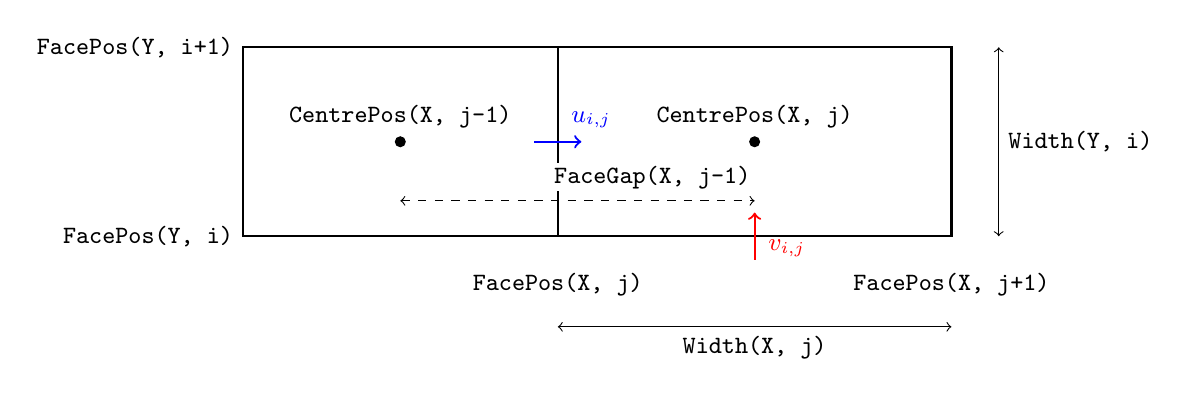
\begin{tikzpicture}[x=1cm,y=1cm,font=\small]
  \draw[thick] (0,0) rectangle (4,2.4);
  \draw[thick] (4,0) rectangle (9,2.4);
  \fill (2,1.2) circle (2pt);
  \fill (6.5,1.2) circle (2pt);
  \node[above] at (6.5,1.25) {\code{CentrePos(X, j)}};
  \node[above] at (2,1.25) {\code{CentrePos(X, j-1)}};
  \node[below] at (4,-0.35) {\code{FacePos(X, j)}};
  \node[below] at (9,-0.35) {\code{FacePos(X, j+1)}};
  \draw[<->] (4,-1.15) -- node[below] {\code{Width(X, j)}} (9,-1.15);
  \draw[<->,dashed] (2,0.45) -- (6.5,0.45); \node[fill=white,inner sep=1pt] at (5.2,0.75) {\code{FaceGap(X, j-1)}};
  \node[left] at (0,0) {\code{FacePos(Y, i)}};
  \node[left] at (0,2.4) {\code{FacePos(Y, i+1)}};
  \draw[<->] (9.6,0) -- node[right] {\code{Width(Y, i)}} (9.6,2.4);
  \draw[->,thick,blue] (3.7,1.2) -- (4.3,1.2); \node[blue,above right] at (4.05,1.25) {$u_{i,j}$};
  \draw[->,thick,red] (6.5,-0.3) -- (6.5,0.3); \node[red,right] at (6.55,-0.15) {$v_{i,j}$};
\end{tikzpicture}
\end{center}
The figure shows two neighbouring cells $(i, j{-}1)$ and $(i, j)$ of one row in 2D. $u_{i,j}$ sits at
(\code{FacePos(X, j)}, \code{CentrePos(Y, i)}). $v_{i,j}$ sits at (\code{CentrePos(X, j)}, \code{FacePos(Y, i)}). $p$
sits at the centre. \code{FaceGap(X, j-1)} is the mean of the widths of cells \code{j-1} and \code{j}. It is the
distance $d_f$ of face $j$ in the pressure coefficient $A_f/d_f$.

\begin{lstlisting}[style=sig]
double Width(Axis a, int n) const;
\end{lstlisting}
The width of a cell along an axis.
\begin{params}
\p{a}{the axis, \code{MAC::X}, \code{Y} or \code{Z}.}
\p{n}{the cell index along that axis (\code{j}, \code{i} or \code{k}).}
\end{params}
\returns{the width, in metres.}

\begin{lstlisting}[style=sig]
double FacePos(Axis a, int n) const;
\end{lstlisting}
The position of a face, the low face of cell \code{n}.
\begin{params}
\p{a}{the axis.}
\p{n}{the face index along that axis, from 0 to the number of cells.}
\end{params}
\returns{the coordinate, in metres.}

\begin{lstlisting}[style=sig]
double CentrePos(Axis a, int n) const;
\end{lstlisting}
The position of the centre of a cell.
\begin{params}
\p{a}{the axis.}
\p{n}{the cell index along that axis.}
\end{params}
\returns{the coordinate, in metres.}

\begin{lstlisting}[style=sig]
double FaceGap(Axis a, int n) const;
\end{lstlisting}
The distance between the centres of cells \code{n} and \code{n+1}, the $d_f$ of the face between them.
\begin{params}
\p{a}{the axis.}
\p{n}{the cell index along that axis.}
\end{params}
\returns{the distance, in metres.}

\begin{lstlisting}[style=sig]
const std::vector<double> &Faces(Axis a) const;
const std::vector<double> &Centres(Axis a) const;
\end{lstlisting}
The whole face table or centre table of an axis, for code that searches or plots it.
\begin{params}
\p{a}{the axis.}
\end{params}
\returns{a read-only reference to the table.}

\begin{lstlisting}[style=sig]
double CellVolume(int i, int j, int k) const;
\end{lstlisting}
The volume of a cell. In 2D it is an area.
\begin{params}
\p{i, j, k}{the cell. The 2D form drops \code{k}.}
\end{params}
\returns{the volume, in cubic metres (square metres in 2D).}

\begin{lstlisting}[style=sig]
double FaceArea(Axis a, int i, int j, int k) const;
\end{lstlisting}
The area of a cell's faces normal to an axis. In 2D it is a length.
\begin{params}
\p{a}{the axis the faces are normal to.}
\p{i, j, k}{the cell. The 2D form drops \code{k}.}
\end{params}
\returns{the area, in square metres (metres in 2D).}
\example
\begin{lstlisting}[style=ex]
// Net volume flux out of cell (i, j, k), correct on a stretched grid
double flux = (g.GetU(i, j + 1, k) - g.GetU(i, j, k)) * g.FaceArea(MAC::X, i, j, k)
            + (g.GetV(i + 1, j, k) - g.GetV(i, j, k)) * g.FaceArea(MAC::Y, i, j, k)
            + (g.GetW(i, j, k + 1) - g.GetW(i, j, k)) * g.FaceArea(MAC::Z, i, j, k);
\end{lstlisting}

\subsection{Field access}

\begin{lstlisting}[style=sig]
double GetU(int i, int j, int k);
double GetV(int i, int j, int k);
double GetW(int i, int j, int k);
double GetP(int i, int j, int k);
void SetU(int i, int j, int k, double value);
void SetV(int i, int j, int k, double value);
void SetW(int i, int j, int k, double value);
void SetP(int i, int j, int k, double value);
\end{lstlisting}
Read or write one stored value of a field. The 2D forms drop \code{k} and have no \code{W}.
\begin{params}
\p{i, j, k}{the face (velocity) or the cell (pressure). See the staggering convention.}
\p{value}{the value to store.}
\end{params}
\returns{the stored value (\code{Get}).}

\begin{lstlisting}[style=sig]
double GetComponent(Component c, int i, int j, int k);
void SetComponent(Component c, int i, int j, int k, double value);
\end{lstlisting}
The same, with the field chosen at run time.
\begin{params}
\p{c}{\code{MAC::U}, \code{V}, \code{W} or \code{P}.}
\p{i, j, k}{the face or the cell. The 2D form drops \code{k}.}
\p{value}{the value to store.}
\end{params}
\returns{the stored value (\code{GetComponent}).}
\example
\begin{lstlisting}[style=ex]
for (MAC::Component c : {MAC::U, MAC::V})
    g.SetComponent(c, i, j, 0.0);
\end{lstlisting}

\begin{lstlisting}[style=sig]
VectorXd &Field(Component c);
const VectorXd &Field(Component c) const;
\end{lstlisting}
The whole array of a field, for work on all values at once, such as copies and norms.
\begin{params}
\p{c}{\code{MAC::U}, \code{V}, \code{W} or \code{P}.}
\end{params}
\returns{a reference to the array.}

\begin{lstlisting}[style=sig]
void ClearFlowFields();
\end{lstlisting}
Sets the velocity and the pressure to zero.

\begin{lstlisting}[style=sig]
void CopyFlowFields(MAC &grid);
void CopyScalarFields(MAC &grid);
void CopyGrid(MAC &grid);
\end{lstlisting}
Copy another grid of the same size into this one. \code{CopyFlowFields} copies the velocity, the pressure and the cell
types. \code{CopyScalarFields} copies the registered scalars, matched by name. \code{CopyGrid} does both.
\begin{params}
\p{grid}{the grid to copy from.}
\end{params}

\subsection{Cells and faces}

\begin{lstlisting}[style=sig]
int GetSolid(int i, int j, int k) const;
void SetSolid(int i, int j, int k, int value);
\end{lstlisting}
Read or write the type of a cell. Changing whether a cell is solid, or changing a ring cell, makes the grid record
its boundary lists again on their next use.
\begin{params}
\p{i, j, k}{the cell. The 2D form drops \code{k}.}
\p{value}{a cell type, \code{FLUID_CELL} to \code{OUTFLOW_CELL}.}
\end{params}
\returns{the cell type (\code{GetSolid}).}

\begin{lstlisting}[style=sig]
enum class GateState { OPEN, WALL, FREE };
\end{lstlisting}
How a cell, or a face, connects the two control volumes on either side of it. The two functions below return it.
\code{OPEN} is fluid to fluid. \code{WALL} is through a solid. \code{FREE} is through air, an inlet or a pressure
cell.

\begin{lstlisting}[style=sig]
GateState CellGate(int i, int j, int k) const;
\end{lstlisting}
How a cell connects its neighbours.
\begin{params}
\p{i, j, k}{the cell. The 2D form drops \code{k}.}
\end{params}
\returns{\code{WALL} for a solid cell, \code{OPEN} for a fluid cell, \code{FREE} otherwise.}

\begin{lstlisting}[style=sig]
GateState FaceGate(Component c, int i, int j, int k) const;
\end{lstlisting}
How a face connects the two cells on either side of it.
\begin{params}
\p{c}{the velocity component the face belongs to.}
\p{i, j, k}{the face. The 2D form drops \code{k}.}
\end{params}
\returns{\code{WALL} if either cell is solid, \code{OPEN} if both are fluid, \code{FREE} otherwise.}
\example
\begin{lstlisting}[style=ex]
if (g.FaceGate(MAC::U, i, j) == GateState::OPEN)   // both cells fluid: solve this face
    ...
\end{lstlisting}

\begin{lstlisting}[style=sig]
bool IsFluidFace(Component c, int i, int j, int k) const;
\end{lstlisting}
Whether the flow is solved on a face.
\begin{params}
\p{c}{the velocity component the face belongs to.}
\p{i, j, k}{the face. The 2D form drops \code{k}.}
\end{params}
\returns{true when the face touches no solid and at least one fluid cell.}

\begin{lstlisting}[style=sig]
bool IsInteriorFluid(int i, int j, int k) const;
\end{lstlisting}
Whether a cell is fluid and inside the domain.
\begin{params}
\p{i, j, k}{the cell. The 2D form drops \code{k}.}
\end{params}
\returns{true for a fluid cell that is not on the ring.}

\begin{lstlisting}[style=sig]
bool IsCellType(int i, int j, int k, int type) const;
\end{lstlisting}
Whether a cell has a given type.
\begin{params}
\p{i, j, k}{the cell. The 2D form drops \code{k}.}
\p{type}{a cell type, \code{FLUID_CELL} to \code{OUTFLOW_CELL}.}
\end{params}
\returns{true when \code{GetSolid(i, j, k) == type}.}

\begin{lstlisting}[style=sig]
int BoundaryKindAt(int i, int j, int k) const;
\end{lstlisting}
The boundary kind of a cell. The three walls share \code{SOLID_CELL}, so the cell type alone cannot tell a no-slip,
a slip and a moving wall apart; the kind can. A ring cell takes the kind of the face that owns it (the scene's,
Section~\ref{sec:mac-bc}); an interior solid is a no-slip wall.
\begin{params}
\p{i, j, k}{the cell. The 2D form drops \code{k}.}
\end{params}
\returns{a \code{BoundaryKind} (\code{BC_NOSLIP} to \code{BC_OUTFLOW}), or $-1$ for an interior cell that is not
solid.}

\begin{lstlisting}[style=sig]
bool IsFluid(int i, int j, int k) const;           // FLUID_CELL
bool IsSolidWall(int i, int j, int k) const;       // SOLID_CELL: any wall or obstacle
bool IsNoSlipWall(int i, int j, int k) const;      // kind BC_NOSLIP (and every obstacle)
bool IsSlipWall(int i, int j, int k) const;        // kind BC_SLIP
bool IsMovingWall(int i, int j, int k) const;      // kind BC_MOVING
bool IsInlet(int i, int j, int k) const;           // INFLOW_CELL
bool IsOutflow(int i, int j, int k) const;         // OUTFLOW_CELL
bool IsPressureOutlet(int i, int j, int k) const;  // EMPTY_CELL or PRESSURE_CELL
\end{lstlisting}
Shorthands for the common questions, built on \code{IsCellType} and \code{BoundaryKindAt}. \code{IsPressureOutlet}
is true for a cell whose pressure is known: a pressure-outlet ring cell, at $p = 0$ (\code{EMPTY_CELL}) or at a
prescribed value (\code{PRESSURE_CELL}). Under a particle method an air cell is also \code{EMPTY_CELL}, at the
free-surface value $p = 0$, so it answers true as well.
\begin{params}
\p{i, j, k}{the cell. The 2D forms drop \code{k}.}
\end{params}
\returns{true when the cell is of that kind.}
\example
\begin{lstlisting}[style=ex]
// the coefficient of a neighbour in a pressure stencil
const double c = g->IsFluid(ni, nj) ? 1.0 : (g->IsPressureOutlet(ni, nj) ? 2.0 : 0.0);
\end{lstlisting}

\begin{lstlisting}[style=sig]
void ResetFluidCells();
\end{lstlisting}
Sets every cell that is not a solid, an inlet, an outflow or a pressure cell to \code{EMPTY_CELL}. A particle method
calls it before it marks the cells that hold particles.

\subsection{Boundaries, sources and initial state}\label{sec:mac-bc}

Each face of the domain has a boundary kind (\code{BoundaryKind} in \code{Definitions.h}): \code{noslip},
\code{slip}, \code{moving}, \code{inlet}, \code{pressure_outlet} or \code{outflow}. The grid imposes a condition by
writing values into the ring of cells outside the domain, either a prescribed value or a copy of the value inside
(zero gradient). Each solver then reads the ring as it needs. A ring cell on an edge or a corner lies on two or three
faces. It takes the kind of the face the scene declares last.

The particle methods (FLIP and SPH) support closed domains with fixed walls only: they do not inject particles at an
inlet or remove them at an outlet, and their contact treats every wall as stationary. The setup screen warns when a
particle method is given an \code{inlet}, \code{outflow}, \code{pressure_outlet} or \code{moving} face.

\begin{ktab}{\linewidth}{@{}>{\raggedright}p{0.17\linewidth} >{\raggedright}p{0.19\linewidth} >{\raggedright}p{0.19\linewidth} >{\raggedright}p{0.16\linewidth} X@{}}
\toprule
\textbf{Kind} & \textbf{Ring cell} & \textbf{Normal velocity} & \textbf{Tangential velocity} & \textbf{Pressure} \\
\midrule
\code{noslip} & \code{SOLID_CELL} & $u_n = 0$ & $u_t = 0$ & copied from inside \\
\midrule
\code{moving} & \code{SOLID_CELL} & $u_n = 0$ & $u_t = U_w(\mathbf x, t)$ & copied from inside \\
\midrule
\code{slip} & \code{SOLID_CELL} & $u_n = 0$ & copied from inside & copied from inside \\
\midrule
\code{inlet} & \code{INFLOW_CELL} & $u_n = g_n(\mathbf x, t)$ & $u_t = g_t(\mathbf x, t)$ & copied from inside \\
\midrule
\code{pressure_outlet} & \code{EMPTY_CELL}; \code{PRESSURE_CELL} with \code{p=} & copied, then set by the projection
  & copied from inside & $p_b(\mathbf x, t)$ on the boundary face, 0 without \code{p=} \\
\midrule
\code{outflow} & \code{OUTFLOW_CELL} & copied, then shifted to match the inlets & copied from inside & copied from
  inside \\
\bottomrule
\end{ktab}

\begin{lstlisting}[style=sig]
void SetBoundaryFunctions(Vec3 (*velocity)(double, double, double, double),
                          double (*pressure)(double, double, double, double));
void SetBoundaryFunctions(Vec2 (*velocity)(double, double, double),
                          double (*pressure)(double, double, double));
\end{lstlisting}
Gives the grid the functions the prescribed boundary values come from. A run gets them from the scene.
\begin{params}
\p{velocity}{the velocity at \code{(x, y[, z], t)}.}
\p{pressure}{the pressure at \code{(x, y[, z], t)}. It is used on a pressure outlet.}
\end{params}

\begin{lstlisting}[style=sig]
void EnforceVelocityBC(double t);
void EnforcePressureBC(double t);
void EnforceBoundaryConditions(double t);
\end{lstlisting}
Apply the boundary conditions at time \code{t}. \code{EnforceVelocityBC} writes the velocity of the ring and of the
boundary faces (below). \code{EnforcePressureBC} writes the ring pressure. \code{EnforceBoundaryConditions} calls
both. A momentum step calls \code{EnforceVelocityBC}. The pressure solver calls \code{EnforcePressureBC}: under the
incremental scheme it restores the ring pressure after the projection, where copying the outlet velocity again would
undo the projection.
\begin{params}
\p{t}{the time the prescribed values are evaluated at, in seconds.}
\end{params}
\example
\begin{lstlisting}[style=ex]
sweepGrid.CopyFlowFields(*gridAnt);
sweepGrid.EnforceVelocityBC(time);    // before the sweep reads its neighbours
\end{lstlisting}

\begin{lstlisting}[style=sig]
double WallLinkFactor(Component c, Axis a, int i, int j, int k, int s) const;
\end{lstlisting}
The wall factor $f_{\mathrm{wall}}$ (below) of the viscous coupling between a face and its neighbour along a
tangential axis. Call it after \code{EnforceVelocityBC}.
\begin{params}
\p{c}{the velocity component the face belongs to.}
\p{a}{the axis of the neighbour, tangential to the component.}
\p{i, j, k}{the face. The 2D form drops \code{k}.}
\p{s}{the side of the neighbour, $-1$ or $+1$.}
\end{params}
\returns{1 unless the neighbour is the value of a no-slip or moving wall. For such a neighbour,
  \code{FaceGap/(Width/2)} of the face's own cell along \code{a}. At a wall of the domain this is exactly 2 on every
  grid, stretched included, because the ring cell is as wide as the interior cell beside it. At the face of an
  obstacle on a stretched grid it is $(W_f + W_s)/W_f$, with $W_f$ the width of the face's cell and $W_s$ that of the
  solid cell.}

\begin{lstlisting}[style=sig]
void AddForce(double time, double dt);
\end{lstlisting}
Adds the body force times \code{dt} to every face that carries fluid, leaving out the faces the boundary sets. The
force is the config's \code{Fu}, \code{Fv} and \code{Fw} plus the scene's \code{force} expression, in units of an
acceleration. Nothing happens when the total force is zero.
\begin{params}
\p{time}{the time at which the scene force is evaluated. This is the start of the step.}
\p{dt}{the time step.}
\end{params}

\begin{lstlisting}[style=sig]
void ApplyInitialField();
\end{lstlisting}
Sets the velocity from the scene's \code{initial} expression at the staggered points. Nothing happens when the scene
has none.

\subsubsection*{The ring and the boundary face}

The figure shows the high end of the $x$ axis in 2D. The last interior cell is $N_x{-}2$ and the ring cell is
$N_x{-}1$. $u_{N_x-2}$ is inside the domain, $u_{N_x-1}$ lies on the boundary face, and $u_{N_x}$ is the outer face of
the ring cell. The ring cell's centre, where its pressure and its tangential velocity are stored, is half a cell
outside the boundary face. The low end mirrors this, with the ring cell 0, the boundary face $u_1$ and the outer face
$u_0$.

\begin{center}
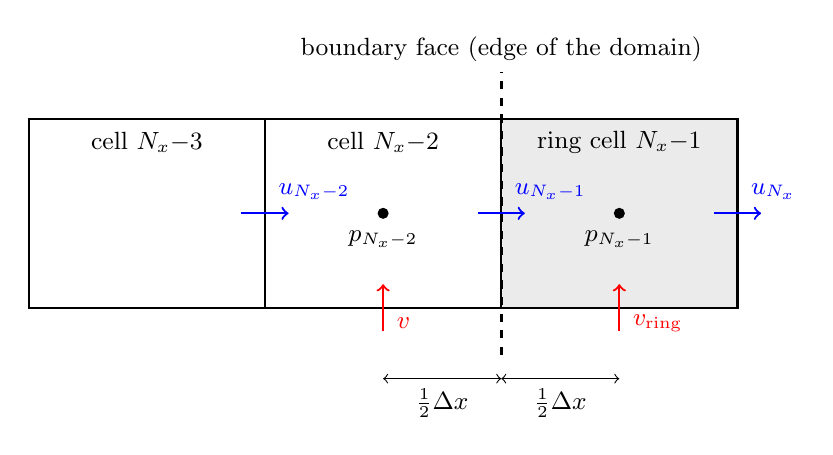
\begin{tikzpicture}[x=1cm,y=1cm,font=\small]
  \fill[black!8] (6,0) rectangle (9,2.4);
  \draw[thick] (0,0) rectangle (3,2.4);
  \draw[thick] (3,0) rectangle (6,2.4);
  \draw[thick] (6,0) rectangle (9,2.4);
  \draw[very thick,dashed] (6,-0.6) -- (6,3.0);
  \node[above] at (6,3.0) {boundary face (edge of the domain)};
  \node at (1.5,2.1) {cell $N_x{-}3$};
  \node at (4.5,2.1) {cell $N_x{-}2$};
  \node at (7.5,2.1) {ring cell $N_x{-}1$};
  \fill (4.5,1.2) circle (2pt); \node[below] at (4.5,1.1) {$p_{N_x-2}$};
  \fill (7.5,1.2) circle (2pt); \node[below] at (7.5,1.1) {$p_{N_x-1}$};
  \draw[->,thick,blue] (2.7,1.2) -- (3.3,1.2); \node[blue,above right] at (3.05,1.25) {$u_{N_x-2}$};
  \draw[->,thick,blue] (5.7,1.2) -- (6.3,1.2); \node[blue,above right] at (6.05,1.25) {$u_{N_x-1}$};
  \draw[->,thick,blue] (8.7,1.2) -- (9.3,1.2); \node[blue,above right] at (9.05,1.25) {$u_{N_x}$};
  \draw[->,thick,red] (4.5,-0.3) -- (4.5,0.3); \node[red,right] at (4.55,-0.2) {$v$};
  \draw[->,thick,red] (7.5,-0.3) -- (7.5,0.3); \node[red,right] at (7.55,-0.2) {$v_{\mathrm{ring}}$};
  \draw[<->] (4.5,-0.9) -- node[below] {$\tfrac{1}{2}\Delta x$} (6,-0.9);
  \draw[<->] (6,-0.9) -- node[below] {$\tfrac{1}{2}\Delta x$} (7.5,-0.9);
\end{tikzpicture}
\end{center}

\subsubsection*{Velocity}

\code{EnforceVelocityBC(t)} runs four passes in this order.
\begin{enumerate}[itemsep=1pt,topsep=2pt]
\item Every face that touches a \code{SOLID_CELL} gets a zero normal velocity, on the walls of the domain and on every
  face of an obstacle.
\item The prescribed values are written, from the velocity function evaluated at the face position and at \code{t}.
  Along the face's normal the grid writes the boundary face and the outer face ($u_1$ and $u_0$ at $x_{\min}$). Along
  the other axes it writes the ring value ($v$ in ring column 0).
\item The zero-gradient copies are written. Normal components copy inward, $u_{N_x-1}$ from $u_{N_x-2}$ and then
  $u_{N_x}$ from $u_{N_x-1}$. A tangential component copies its interior neighbour, $v_{\mathrm{ring}}$ from $v$.
  Faces are copied first, then edges, then corners, so a corner copies from an edge that is already set.
\item At a continuity outflow the flux is corrected to match the inlets (below).
\end{enumerate}

\subsubsection*{No-slip and moving walls}

The ring stores the wall velocity $u_w$ at the centre of the ring cell, but the wall is the boundary face, half a cell
closer. So the viscous coupling between the first interior face $u_1$ and the ring is half a cell long. The viscous
flux through the wall is
\begin{equation*}
  \nu\,\frac{u_w - u_1}{\Delta/2} \;=\; \nu\,\frac{u_g - u_1}{\Delta}, \qquad u_g = 2u_w - u_1 ,
\end{equation*}
the same as a ghost value $u_g$ reflected through the wall (Harlow and Welch 1965). The coefficient of that coupling
is multiplied by
\begin{equation*}
  f_{\mathrm{wall}} = \frac{\code{FaceGap}}{\code{Width}/2},
\end{equation*}
which is 2 on a uniform grid. \code{WallLinkFactor} returns it, and 1 on every coupling that does not end in a no-slip
or moving wall, a slip wall included. It holds on the walls of the domain and on every face of an obstacle.

\begin{center}
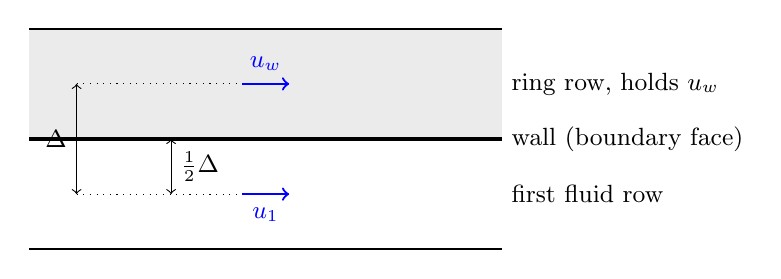
\begin{tikzpicture}[x=1cm,y=1cm,font=\small]
  \fill[black!8] (0,2.8) rectangle (6,4.2);
  \draw[thick] (0,1.4) -- (6,1.4); \draw[very thick] (0,2.8) -- (6,2.8); \draw[thick] (0,4.2) -- (6,4.2);
  \node[right] at (6,2.8) {wall (boundary face)};
  \node[right] at (6,3.5) {ring row, holds $u_w$};
  \node[right] at (6,2.1) {first fluid row};
  \draw[->,thick,blue] (2.7,3.5) -- (3.3,3.5); \node[blue,above] at (3,3.55) {$u_w$};
  \draw[->,thick,blue] (2.7,2.1) -- (3.3,2.1); \node[blue,below] at (3,2.05) {$u_1$};
  \draw[dotted] (0.6,2.1) -- (2.7,2.1); \draw[dotted] (0.6,3.5) -- (2.7,3.5);
  \draw[<->] (1.8,2.1) -- node[right] {$\tfrac{1}{2}\Delta$} (1.8,2.8);
  \draw[<->] (0.6,2.1) -- node[left] {$\Delta$} (0.6,3.5);
\end{tikzpicture}
\end{center}

\subsubsection*{Continuity outflow}

After the copies, the outflow faces carry the interior flux, which need not equal the inflow. Let $s = \pm 1$ be the
sign of the outward normal of a face, $u$ its normal velocity and $A$ its area. The grid sums
\begin{equation*}
  Q_{\mathrm{in}} = -\sum_{\text{inlet faces}} s\,u\,A, \qquad
  Q_{\mathrm{out}} = \sum_{\text{outflow faces}} s\,u\,A, \qquad
  A_{\mathrm{out}} = \sum_{\text{outflow faces}} A,
\end{equation*}
and adds one uniform correction to every outflow face,
\begin{equation*}
  \delta = \frac{Q_{\mathrm{in}} - Q_{\mathrm{out}}}{A_{\mathrm{out}}}, \qquad
  u \leftarrow u + s\,\delta, \qquad u_{\mathrm{outer}} \leftarrow u .
\end{equation*}
The net flux through the boundary is then zero. To the pressure solve an outflow is a known velocity, like an inlet,
so with no pressure outlet the pressure system is singular and needs \code{NEEDS_COMPATIBILITY_CONDITION}.

\subsubsection*{Pressure}

\code{EnforcePressureBC(t)} sets each ring cell from its type.
\begin{itemize}[itemsep=1pt,topsep=2pt]
\item An \code{EMPTY_CELL}, a pressure outlet without \code{p=}, gets 0.
\item A \code{PRESSURE_CELL} gets the prescribed $p_b(\mathbf x, t)$, evaluated on the boundary face.
\item Any other ring cell copies its interior neighbour, a zero normal gradient.
\end{itemize}

\textbf{At a pressure outlet.} The value $p_b$ belongs on the boundary face, which is half a cell from the centre of
the last fluid cell, not a full cell. The pressure matrix and the projection therefore take the gradient over the
half cell,
\begin{equation*}
  \frac{\partial p}{\partial n}\bigg|_{\mathrm{face}} \approx \frac{p_b - p_{\mathrm{in}}}{\Delta/2},
\end{equation*}
which multiplies the coefficient of that face by $f_{\mathrm{D}} = \code{FaceGap}/(\code{Width}/2)$, 2 on a uniform
grid. A linear pressure field is then exact to round-off. The outlet's normal velocity is first copied from inside;
the projection then corrects it with this gradient, so the flux through the outlet face is divergence free.

\textbf{At a wall or an inlet.} Here the normal velocity $g_n$ is known and the pressure is not. Take the normal
component of the momentum equation on the boundary face, with the derivatives along the face set to zero. Continuity
then gives $\partial u_n/\partial n = 0$, so the convective and the viscous terms vanish, and what the velocity
prescribes for the pressure is
\begin{equation*}
  \frac{\partial p}{\partial n} = \rho\left(f_n - \frac{\partial g_n}{\partial t}\right),
\end{equation*}
the hydrostatic gradient at a wall at rest. The code does not impose this. The boundary face's $u^*$ is set to
$g_n(t^{n+1})$ and the projection does not correct it, so the solve uses the homogeneous condition
\begin{equation*}
  \frac{\partial p}{\partial n} = 0
\end{equation*}
for the projection's pressure (Chorin) or increment (incremental). The force and $\partial g_n/\partial t$ enter
$u^*$ on the interior faces, so the right gradient is recovered inside the domain; the difference is the $O(\Delta t)$
artificial boundary layer of projection methods (Guermond, Minev and Shen 2006). A \code{pressure_inlet} kind, which
would prescribe the pressure and let the normal velocity follow, is not implemented.

% -----------------------------------------------------------------------------------------------------
\subsection{Differential operators}

This part of the interface is small and is being reworked. A future version will offer the gradient, the divergence
and the Laplacian of any field, and a gradient at any physical point, in one consistent set of functions. Until then
a method writes its own stencils from the spacing tables, as the tutorial does.

\begin{lstlisting}[style=sig]
double GetDivergencyAt(int i, int j, int k);
\end{lstlisting}
The discrete divergence of a cell, the net flux through its faces divided by its volume.
\begin{params}
\p{i, j, k}{the cell. The 2D form drops \code{k}.}
\end{params}
\returns{the divergence, in 1/s. It is zero for a cell that is not fluid.}

\begin{lstlisting}[style=sig]
double GetGradP(Axis a, int i, int j, int k);
double GetGradP(Axis a, int i, int j);
\end{lstlisting}
The pressure gradient on the low face of a cell along an axis, where \code{u}, \code{v} or \code{w} sits: the
difference of the two cell pressures divided by \code{FaceGap}, the same $d_f$ the pressure matrix uses.
\begin{params}
\p{a}{the axis of the face.}
\p{i, j, k}{the cell whose low face it is. The 2D form drops \code{k}.}
\end{params}
\returns{the gradient, in Pa/m. It is not defined on the outermost faces.}

\subsection{Interpolation and sampling}

\begin{lstlisting}[style=sig]
double ComponentAtFace(Component c, Component target, int i, int j, int k);
double getVatU(int i, int j, int k);   // also getWatU, getUatV, getWatV, getUatW, getVatW
\end{lstlisting}
One velocity component where another is stored. It averages four values, over the two faces of \code{c} along its
axis and the two cells along the axis of \code{target}, weighted by distance on a stretched grid. The
\code{getXatY} forms are short names, so \code{getVatU} is \code{v} at a \code{u} face.
\begin{params}
\p{c}{the component to sample.}
\p{target}{the component whose face \code{(i, j, k)} is the sample point.}
\p{i, j, k}{the face. The 2D form drops \code{k}.}
\end{params}
\returns{the interpolated value.}

\begin{lstlisting}[style=sig]
double ComponentAt(Component c, double x, double y, double z);
\end{lstlisting}
A field at a physical point, by trilinear interpolation (bilinear in 2D). A velocity component is interpolated over
its own faces along its axis and over the nearest cell centres along the others. The pressure is interpolated over
the cell centres. The interpolation does not look at the cell types, so a caller that must not read a solid checks
for one itself.
\begin{params}
\p{c}{\code{MAC::U}, \code{V}, \code{W} or \code{P}.}
\p{x, y, z}{the point, in metres. The 2D form drops \code{z}.}
\end{params}
\returns{the interpolated value. Beyond the first and the last centre it is constant.}

\begin{lstlisting}[style=sig]
double ScalarAt(int handle, double x, double y, double z);
double ScalarAt(const std::string &name, double x, double y, double z);
\end{lstlisting}
A registered scalar at a point, sampled in the same way as the pressure.
\begin{params}
\p{handle, name}{the scalar, by its handle or by its name.}
\p{x, y, z}{the point, in metres.}
\end{params}
\returns{the interpolated value, or 0 for a scalar the grid does not carry.}
\example
\begin{lstlisting}[style=ex]
const double p = g.ComponentAt(MAC::P, 0.45, 0.20, 0.205);
const double d = g.ScalarAt("d", 0.45, 0.20, 0.205);
\end{lstlisting}

\begin{lstlisting}[style=sig]
int CellAt(Axis axis, double x) const;
\end{lstlisting}
The cell that holds a coordinate along one axis. There is no single call from a point to \code{(i, j, k)}: call it
once per axis, \code{MAC::X} for \code{j}, \code{MAC::Y} for \code{i} and \code{MAC::Z} for \code{k}. \code{CentrePos}
goes back from an index to a coordinate.
\begin{params}
\p{axis}{the axis.}
\p{x}{the coordinate, in metres.}
\end{params}
\returns{the cell index along that axis. A coordinate outside the grid gives the first or the last cell.}
\example
\begin{lstlisting}[style=ex]
const int j = g.CellAt(MAC::X, x), i = g.CellAt(MAC::Y, y);   // the cell holding the point (x, y)
const double p = g.GetP(i, j);
\end{lstlisting}

\subsection{Diagnostics}

\begin{lstlisting}[style=sig]
bool AllFinite() const;
\end{lstlisting}
Checks every value of the velocity and the pressure. The shipped program calls it after every step and ends a run
whose field is not finite.
\returns{true when all of them are finite.}

\begin{lstlisting}[style=sig]
double GetMaxVelocity();
\end{lstlisting}
The largest speed of the velocity, taken at the cell centres. A NaN does not change it, so use \code{AllFinite} to
detect a blown-up field.
\returns{the speed, in m/s.}

\begin{lstlisting}[style=sig]
double GetDivSum();
\end{lstlisting}
The sum of the absolute divergence over the interior cells, the divergence the telemetry reports.
\returns{the sum.}

\begin{lstlisting}[style=sig]
int GetFluidCellCount();
\end{lstlisting}
\returns{the number of fluid cells.}

\begin{lstlisting}[style=sig]
double MaxAbsoluteDifference(MAC &grid);
\end{lstlisting}
The largest change in the velocity between this grid and another, the step residual.
\begin{params}
\p{grid}{a grid of the same size.}
\end{params}
\returns{the largest absolute difference in \code{u}, \code{v} or \code{w}.}

\subsection{Scalar registry}

A grid can carry cell-centred scalars, such as a density, a temperature or a tracer. Each one is registered by name.
It is sized and indexed like \code{p}. Copies, checkpoints and exports carry it.

\begin{lstlisting}[style=sig]
int RegisterScalar(const std::string &name, TransportScheme scheme = TransportScheme::Upwind);
int RegisterScalar(const std::string &name, const ScalarTransport &transport);
\end{lstlisting}
Adds a field of zeros. A second call with the same name returns the same handle and keeps the first transport, and a
different transport in the second call is reported.
\begin{params}
\p{name}{the name of the field.}
\p{scheme, transport}{how the transport solver moves it: the scheme alone, or the solver, scheme, form,
  diffusivity and reaction rate. A \code{transport.solver} of \code{ScalarSolver::None} leaves the field to the
  method: the transport step only sets its ring.}
\end{params}
\returns{the handle of the field.}
\example
\begin{lstlisting}[style=ex]
int d = g.RegisterScalar("d");
g.SetS(d, i, j, k, 1.0);
\end{lstlisting}

\begin{lstlisting}[style=sig]
int ScalarHandle(const std::string &name) const;
\end{lstlisting}
\begin{params}
\p{name}{the name of the field.}
\end{params}
\returns{the handle of the field, or $-1$ when the grid does not carry it.}

\begin{lstlisting}[style=sig]
int ScalarCount() const;
const std::string &ScalarName(int h) const;
\end{lstlisting}
\begin{params}
\p{h}{a handle, from 0 to \code{ScalarCount() - 1}.}
\end{params}
\returns{the number of fields, and the name of field \code{h}.}

\begin{lstlisting}[style=sig]
const ScalarTransport &ScalarTransportOf(int h) const;
\end{lstlisting}
\begin{params}
\p{h}{the handle of the field.}
\end{params}
\returns{the field's solver, scheme, form, diffusivity and reaction rate.}

\begin{lstlisting}[style=sig]
void EnforceScalarBC(int h, double t);
\end{lstlisting}
Sets the ring of field \code{h}: on a face where the scene pins the scalar, the scene's value at time \code{t}; on
every other ring cell, a copy of the cell inside (zero gradient). The transport step calls it after each solve, and
for a field with no solver (\code{solver=none}) it is all the step does, so a method that updates such a field itself
(a turbulence model, say) finds the boundary values in the ring.
\begin{params}
\p{h}{the handle of the field.}
\p{t}{the time the scene's value is evaluated at.}
\end{params}

\begin{lstlisting}[style=sig]
double ScalarSourceAt(int h, double x, double y, double z, double t) const;
\end{lstlisting}
Evaluates field \code{h}'s \code{source} expression from the scene. The ADI transport solver applies it once per
step, before its sweeps, at each fluid cell centre; a method updating a field with no solver calls this to do the
same. Call it from serial code only: the expression's variables live at fixed addresses, so two threads evaluating it
at once overwrite each other's.
\begin{params}
\p{h}{the handle of the field.}
\p{x, y, z}{the point, in metres. In 2D \code{z} is ignored.}
\p{t}{the time, in seconds.}
\end{params}
\returns{$S(x, y, z, t)$, or 0 when the field has no source.}

\begin{lstlisting}[style=sig]
double GetS(int h, int i, int j, int k) const;
void SetS(int h, int i, int j, int k, double value);
\end{lstlisting}
Read or write one value of a field, at a cell centre.
\begin{params}
\p{h}{the handle of the field.}
\p{i, j, k}{the cell. The 2D form drops \code{k}.}
\p{value}{the value to store.}
\end{params}
\returns{the stored value (\code{GetS}).}

\begin{lstlisting}[style=sig]
VectorXd &ScalarField(int h);
\end{lstlisting}
\begin{params}
\p{h}{the handle of the field.}
\end{params}
\returns{a reference to the whole array of the field, indexed like \code{p}.}

\begin{lstlisting}[style=sig]
void ClearScalars();
\end{lstlisting}
Removes every registered field.

% =====================================================================================================
\section{Methods, settings and steps (Definitions.h)}\label{sec:registry}

\code{src/headers/Core/Definitions.h} holds the types a method author needs: the method row, the capability bits,
the settings tables and the step list.

\subsection{The method row}

\begin{lstlisting}[style=sig]
struct SimulationMethod {
    const char *key;
    const char *label;
    const char *help;
    MethodFamily family;
    bool supports2D;
    bool supports3D;
    unsigned caps;
    void (*initialize)();
    void (*dispose)();
    void *settings;
    const SettingField *settingFields;
    int settingCount;
    void (*drawSettings)(const SettingsContext &ctx);
    void (*checkSettings)(const SettingsContext &ctx, std::vector<std::string> &problems,
                          std::vector<std::string> &notes);
    double (*stableTimestep)();
    double (*maxVelocity)();
    double (*cflLength)();
    double (*particleSpacing)();
};
\end{lstlisting}
Everything the program knows about a method. \code{key} is the value of \code{TYPE} in the config, the prefix of its
settings block (\code{<KEY>_BEGIN}), and the tag in a checkpoint. It may be 1 to 63 characters long
(\code{MAX_METHOD_KEY} $- 1$), the size of the checkpoint's key field. The setup screen shows \code{label} and \code{help}. \code{initialize} builds the method's solvers and
registers its steps (Section~\ref{sec:steps-api}). \code{dispose} frees what \code{initialize} allocated; it may be
null when the method holds nothing worth freeing. The settings members point at the method's settings struct and at
its table (Section~\ref{sec:settings-api}). \code{drawSettings} and \code{checkSettings} are optional hooks for the
setup screen. The last four members are optional questions. A null pointer means the manager answers from the grid.
\begin{params}
\p{family}{\code{MethodFamily::EULERIAN}, \code{HYBRID} or \code{LAGRANGIAN}. The family groups the method on the
  setup screen and limits its capabilities.}
\p{caps}{the capability bits below, combined with OR. They must stay within what the family offers.}
\p{stableTimestep}{the method's own largest stable step. It is used under \code{ADAPTATIVE_TIMESTEP}.}
\p{maxVelocity, cflLength}{the speed and the length for the CFL number, for a method whose grid does not carry them.}
\p{particleSpacing}{the distance between seeded particles. The surface export uses it.}
\end{params}

\begin{lstlisting}[style=sig]
enum MethodCapability : unsigned {
    CAP_GRID, CAP_PARTICLES, CAP_RECTILINEAR, CAP_BOUNDARY_CELLS,
    CAP_FIXED_REGION, CAP_SCALARS, CAP_PRESSURE_SOLVER };
\end{lstlisting}
Each capability is one bit of a mask, so a row lists what it supports by combining them with \code{|}.
\begin{itemize}[itemsep=0pt,topsep=1pt]
\item \code{CAP_GRID}. A MAC grid carries the solution, so there are field views and \code{.vtr} exports.
\item \code{CAP_PARTICLES}. There is a particle set to draw and export.
\item \code{CAP_RECTILINEAR}. The method can run on a stretched grid.
\item \code{CAP_BOUNDARY_CELLS}. The border is a ring of boundary cells.
\item \code{CAP_FIXED_REGION}. The fluid region does not move.
\item \code{CAP_SCALARS}. The registered scalars are transported.
\item \code{CAP_PRESSURE_SOLVER}. The method uses the shared pressure solver (Section~\ref{sec:pressure-api}), so the
  setup screen shows the settings of that solver.
\end{itemize}
\example
\begin{lstlisting}[style=ex]
// An Eulerian method on stretched grids, with the shared pressure solver and no scalars
const unsigned caps = CAP_GRID | CAP_RECTILINEAR | CAP_BOUNDARY_CELLS | CAP_FIXED_REGION | CAP_PRESSURE_SOLVER;
if (caps & CAP_SCALARS) { /* never: the bit is not set */ }
\end{lstlisting}
A family is an upper limit. A row that claims a bit its family does not offer is refused when it is registered.
\begin{center}\small
\begin{tabular}{lccccccc}
\toprule
family & grid & particles & rectilinear & boundary cells & fixed region & scalars & shared PPE\\
\midrule
\code{EULERIAN}   & yes & & yes & yes & yes & yes & yes\\
\code{HYBRID}     & yes & yes & & yes & & & yes\\
\code{LAGRANGIAN} & & yes & & & yes & & \\
\bottomrule
\end{tabular}
\end{center}

\begin{lstlisting}[style=sig]
int RegisterSimulationMethod(const SimulationMethod &m);
\end{lstlisting}
Adds a row to the registry. It stops with an error on a key that is empty, longer than 63 characters or already
used, on capabilities outside the family, or when the registry is full (16 rows). Call it before \code{InitializeSimulation}, which looks up the
config's \code{TYPE} here.
\begin{params}
\p{m}{the method's row.}
\end{params}
\returns{the id of the row. \code{SIM_TYPE} holds this id while the method runs.}

\begin{lstlisting}[style=sig]
const SimulationMethod &MethodOf(int id);
\end{lstlisting}
\begin{params}
\p{id}{the id \code{RegisterSimulationMethod} returned.}
\end{params}
\returns{the row. An id out of range gives an empty \code{UNKNOWN} row, so the lookup never fails.}

\begin{lstlisting}[style=sig]
const SimulationMethod &ActiveMethod();
\end{lstlisting}
\returns{the row of the method the config chose, \code{MethodOf(SIM_TYPE)}.}
\example
\begin{lstlisting}[style=ex]
std::printf("running %s\n", ActiveMethod().key);
\end{lstlisting}

\begin{lstlisting}[style=sig]
int MethodFromKey(const std::string &key);
\end{lstlisting}
\begin{params}
\p{key}{a method's key, the value of \code{TYPE} in a config.}
\end{params}
\returns{the id of the row, or $-1$ for an unknown key.}

\begin{lstlisting}[style=sig]
bool MethodSupports(int id, unsigned cap);
\end{lstlisting}
\begin{params}
\p{id}{the id of a row.}
\p{cap}{one capability bit, \code{CAP_GRID} to \code{CAP_PRESSURE_SOLVER}.}
\end{params}
\returns{true when the row sets the bit and its family allows it.}

\begin{lstlisting}[style=sig]
bool MethodUsesGrid();
bool MethodUsesParticles();
bool MethodSupportsRectilinear();
bool MethodUsesBoundaryCells();
bool MethodFixedFluidRegion();
\end{lstlisting}
Shorthands for \code{MethodSupports} on the active method, one capability each. Shared code uses them to decide what
to do without naming a method.
\returns{true when the active method has the capability.}

\begin{lstlisting}[style=sig]
double ActiveMethodSetting(const char *key, double fallback);
\end{lstlisting}
Reads a setting of the active method by its config key. Shared code uses it so that it does not have to name a method.
\begin{params}
\p{key}{the config key of the setting.}
\p{fallback}{the value to return when the active method has no such key.}
\end{params}
\returns{the value of the setting, or \code{fallback}.}

\subsection{Settings tables}\label{sec:settings-api}

A method's settings are a plain struct with one global instance, in the method's own header. A table of
\code{SettingField} rows says where each field sits and what its config key is. The config reader, the config writer
and the setup screen all walk this table, so each key is written in one place only.

\begin{lstlisting}[style=sig]
constexpr SettingField IntSetting(const char *key, const char *label, const char *help,
                                  size_t offset, int def,
                                  double lo = SETTING_NO_MIN, double hi = SETTING_NO_MAX);
constexpr SettingField DoubleSetting(const char *key, const char *label, const char *help,
                                     size_t offset, double def,
                                     double lo = SETTING_NO_MIN, double hi = SETTING_NO_MAX);
constexpr SettingField BoolSetting(const char *key, const char *label, const char *help,
                                   size_t offset, bool def);
constexpr SettingField EnumSetting(const char *key, const char *label, const char *help,
                                   size_t offset, int def,
                                   const char *const *keys, const char *const *labels, int count);
\end{lstlisting}
Each function makes one row. The setup screen draws an integer with both bounds as a slider, a double as an input box
kept inside its range, a bool as a checkbox and an enum as a drop-down list. \code{help} is the tooltip.
\begin{params}
\p{key}{the config key. It is read inside the method's block, between \code{<KEY>_BEGIN} and \code{<KEY>_END}.}
\p{label, help}{the name and the tooltip on the setup screen.}
\p{offset}{\code{offsetof(TheStruct, field)}.}
\p{def, lo, hi}{the default and the range.}
\p{keys, labels, count}{how each enum value is written in the file and shown on screen, in enum order.}
\end{params}
\returns{the row, to put in the method's table.}

\begin{lstlisting}[style=sig]
constexpr SettingField WithUnit(SettingField f, const char *unit);
\end{lstlisting}
The same row with a unit, which the setup screen shows after the value. Rows without one show none.
\begin{params}
\p{f}{a row made by one of the functions above.}
\p{unit}{the unit as it should read, \code{"m"}, \code{"m/s"}, \code{"1/s"}.}
\end{params}
\returns{the row with its unit set.}
\example
\begin{lstlisting}[style=ex]
struct MySettings { double relaxation = 1.7; int maxIterations = 1000; double radius = 0.05; };
inline MySettings MY_SETTINGS;
inline const SettingField MY_FIELDS[] = {
    DoubleSetting("MY_RELAXATION", "Relaxation", "SOR factor, 0.5 to 2",
                  offsetof(MySettings, relaxation), 1.7, 0.5, 2.0),
    IntSetting("MY_MAX_ITERATIONS", "Max sweeps", "", offsetof(MySettings, maxIterations), 1000, 1, 1e7),
    WithUnit(DoubleSetting("MY_RADIUS", "Radius", "", offsetof(MySettings, radius), 0.05, 0.0), "m"),
};
\end{lstlisting}

\begin{lstlisting}[style=sig]
struct SettingsContext {
    int dimension;
    double dh, density, viscosity, timeStep;
    bool adaptiveTimestep;
    double x0, xf, y0, yf, z0, zf, fu, fv, fw, meanVelocity, characteristicLength;
};
\end{lstlisting}
What a method's panel or check is told about the rest of the setup. A panel uses it for read-outs such as a cell
Reynolds number.

\subsection{Steps}\label{sec:steps-api}

\begin{lstlisting}[style=sig]
using SimulationStepFunction = void (*)(MAC *gridAnt, MAC *gridSol,
                                        ParticleSet *particles, double time);
using SimulationStepCounter  = int (*)();
void RegisterSimulationStep(SimulationStepFunction function, const std::string &name, int order,
                            SimulationStepCounter counter = nullptr);
\end{lstlisting}
Adds a step to the list the manager runs every time step. The list is sorted by \code{order}. Steps with the same
order keep their registration order. A method's \code{initialize} calls it. The manager times each step and writes
one telemetry column \code{<name>_timing} per step, so a step needs no timing code.

The optional \code{counter} lets the manager learn a step's iteration count without asking any method for it. After
the step runs, the manager calls it and writes the value in the column \code{<name>_counter}. A step registered
without one reports $-1$. The pressure solver's \code{pressure} step returns the iterations of its last solve. The
counter columns are written with the timing columns, when \code{EXPORT_COLUMN_STEP_TIMINGS} is on.
\begin{params}
\p{gridAnt}{the field at the start of the step. Read it. Do not write it.}
\p{gridSol}{the field the step builds. The manager zeroes it before the first step.}
\p{particles}{the particle set of the run. It is empty for a method without particles.}
\p{time}{the simulated time at the start of the step. \code{SIMULATION.time} holds the time the step solves for.}
\p{order}{the position in the list. The shipped steps use the orders in the table below.}
\p{counter}{a function that returns the step's work count for the step it just ran, or \code{nullptr}.}
\end{params}
A step works only on the grids and particles it is handed, and writes no global state. The manager measures the
divergence after the last step.

\begin{center}\small
\begin{tabular}{@{}rlll@{}}\toprule
order & name & registered by & method \\\midrule
0 & \code{momentum}, \code{particle_advection}, \code{sph} & the method & ADI, FLIP, SPH \\
2 & \code{grid_diffusion} & the method & FLIP \\
4 & \code{pressure} & the pressure solver & ADI, FLIP \\
6 & \code{projection} & the pressure solver & ADI, FLIP \\
7 & \code{grid_to_particle} & the method & FLIP \\
8 & \code{density_correction} & the method, when it is on & FLIP \\
8 & \code{transport} & the transport solver, when there are scalars & ADI \\\bottomrule
\end{tabular}
\end{center}


% =====================================================================================================
\section{The pressure solver (\texorpdfstring{\texttt{Methods/PPESolver/}}{Methods/PPESolver/})}\label{sec:pressure-api}

\code{PressureSolver2D} and \code{PressureSolver3D}, with \code{PressureSettings.h}. A shared solver for the pressure
Poisson equation that any grid method can use. It is not a method and registers no row. The method tells it which
projection scheme it wants, and the solver does the rest: it registers its own steps, builds the matrix from the cell
types, keeps the matrix while the cells do not change, and solves on the CPU (Eigen or AMGCL) or on an NVIDIA GPU
(AMGX). The config's \code{PRESSURE} block chooses the backend. A method that sets \code{CAP_PRESSURE_SOLVER} uses
this solver.

The solve finds the pressure from
\begin{equation*}
  \nabla^2 p = \frac{\rho}{\Delta t}\,\nabla\cdot\mathbf{u}^*,
\end{equation*}
and the projection corrects the velocity on every face that is not a wall,
\begin{equation*}
  \mathbf{u} = \mathbf{u}^* - \frac{\Delta t}{\rho}\,\nabla p .
\end{equation*}
Walls, inlets and outflows give a Neumann condition, a pressure outlet a Dirichlet condition on the boundary face
(Section~\ref{sec:mac-bc}).

\begin{lstlisting}[style=sig]
static void InitializePressureSolver(MAC *grid, PressureScheme scheme = PRESSURE_CHORIN);
\end{lstlisting}
Chooses the backend, builds the matrix, and registers the \code{pressure} step (order 4) and the \code{projection}
step (order 6). Call it once from the method's \code{initialize}. The \code{pressure} step is registered with the
counter \code{LastIterations}, so the telemetry column \code{pressure_counter} holds the iterations of each solve.
\begin{params}
\p{grid}{the grid whose cell types define the system.}
\p{scheme}{\code{PRESSURE_CHORIN} or \code{PRESSURE_INCREMENTAL}. With Chorin the solve returns the pressure. With
  the incremental scheme the momentum step includes the old pressure gradient, the solve returns the increment, and
  the projection adds it to the old pressure.}
\end{params}

\begin{lstlisting}[style=sig]
static int LastIterations();
\end{lstlisting}
The \code{pressure} step's counter (Section~\ref{sec:steps-api}).
\returns{the iterations of the last pressure solve.}

\begin{lstlisting}[style=sig]
static void SolveChorin(MAC *gridAnt, MAC *gridSol, ParticleSet *particles, double time);
static void SolveIncremental(MAC *gridAnt, MAC *gridSol, ParticleSet *particles, double time);
static void SolvePressure(MAC *gridAnt, MAC *gridSol, ParticleSet *particles, double time);
static void Project(MAC *gridAnt, MAC *gridSol, ParticleSet *particles, double time);
\end{lstlisting}
\code{SolveChorin} and \code{SolveIncremental} are the two pressure steps; \code{InitializePressureSolver} registers
one of them. \code{SolvePressure} runs the one it chose, for a program that drives the solver itself. \code{Project}
is the projection step. Under the incremental scheme it also forms the new pressure.
\begin{params}
\p{gridAnt, gridSol, particles, time}{the arguments of every step (Section~\ref{sec:steps-api}). The solve reads the
  divergence of \code{gridSol} and writes the pressure there. The incremental scheme reads the old pressure from
  \code{gridAnt}.}
\end{params}

\begin{lstlisting}[style=sig]
static bool SolveLaplacian(MAC *grid, const VectorXd &f, VectorXd &x);
static int SystemSize();
\end{lstlisting}
\code{SolveLaplacian} solves $L x = f$ on the current fluid cells, with the boundary conditions of the pressure
matrix. It reuses the matrix and its multigrid hierarchy, for a second Poisson solve in the same step. FLIP's density
correction uses it. \code{SystemSize} is the length of the vectors it takes.
\begin{params}
\p{grid}{the grid whose fluid cells define the system.}
\p{f}{the right-hand side, one value per fluid cell.}
\p{x}{the solution, written in place.}
\end{params}
\returns{false when the solve did not converge (\code{SolveLaplacian}), the number of unknowns (\code{SystemSize}).}

\begin{lstlisting}[style=sig]
static void ReleasePressureSolver();
static void DestroyPressureSolver();
\end{lstlisting}
\code{ReleasePressureSolver} frees the matrix, the AMG hierarchy and the AMGX handle, and leaves the AMGX library up;
a method's \code{dispose} calls it, so a later run can use AMGX again. \code{DestroyPressureSolver} does the same and
then shuts AMGX down when no handle is left. A program that used AMGX calls it once, at exit.

% =====================================================================================================
\section{Scalar transport}\label{sec:transport-api}

\code{TransportSolver2D} and \code{TransportSolver3D}, declared in \code{src/headers/Solvers/} and defined in
\code{src/}. They move every scalar $\phi$
the grid carries with the solved velocity, with optional diffusion, reaction and source,
\begin{equation*}
  \frac{\partial\phi}{\partial t} + \mathrm{conv}(\mathbf{u},\phi) = \nabla\cdot(\epsilon\nabla\phi) - \gamma\phi + S .
\end{equation*}
A scalar is declared in the scene (Section~\ref{sec:scene-api}) or registered with \code{MAC::RegisterScalar}. Its
solver, its scheme (central or upwind), its form (flux or advective), $\epsilon$ and $\gamma$ travel with it. A scalar
declared with \code{solver=none} is stored, copied, checkpointed and exported like the others, and its ring is set
every step, but the transport step does not move it: the method that owns it updates the values.

\begin{lstlisting}[style=sig]
static void InitializeTransportSolver2D(MAC *grid);
static void InitializeTransportSolver3D(MAC *grid);
\end{lstlisting}
Sizes the work arrays and registers the \code{transport} step at order 8, after the projection, so the scalars move
with the divergence-free velocity. Call it from the method's \code{initialize} when the grid carries scalars.
\begin{params}
\p{grid}{the grid whose scalars are transported.}
\end{params}

\begin{lstlisting}[style=sig]
static void SolveTransportStep(MAC *gridAnt, MAC *gridSol, ParticleSet *particles, double time);
\end{lstlisting}
The \code{transport} step. It moves every registered scalar one time step.
\begin{params}
\p{gridAnt}{the grid the scalars are read from.}
\p{gridSol}{the grid the new scalars are written to, with the projected velocity that moves them.}
\p{particles, time}{the remaining step arguments. \code{time} is the start of the step.}
\end{params}

% =====================================================================================================
\section{Particles}\label{sec:particles-api}

\code{Definitions.h} holds the particle types. \code{src/headers/Core/Particles.h} holds the operations that every
particle method shares. Particle runs are limited to closed domains with fixed walls: no particle is injected or
removed at a boundary, and every wall is stationary for the contact (Section~\ref{sec:mac-bc}).

\begin{lstlisting}[style=sig]
struct Particle { bool isActive; double x, y, z; double u, v, w; };
struct ParticleSet { std::vector<Particle> data; int count; std::vector<double> density; };
\end{lstlisting}
The particles of a run live in \code{SIMULATION.particles}, and every step receives them. \code{data.size()} is the
capacity, set once by the method's \code{initialize}. The first \code{count} entries are the live particles. In 2D,
\code{z} and \code{w} stay zero. \code{density} is for a method that carries one density per particle between steps
(SPH); it is empty otherwise, and the checkpoint writes it when it is not. Any other data a method needs stays in the
method.

\begin{lstlisting}[style=sig]
void Particles::ResolveContacts(MAC *grid, const Particle &previous, Particle &p);
\end{lstlisting}
Keeps a particle of a grid method out of the walls and the obstacles after it has moved, and applies the contact
response (Section~\ref{sec:contact}). Section~\ref{sec:contact-grid} gives the stages.
\begin{params}
\p{grid}{the grid whose cell types mark the solids.}
\p{previous}{the particle before the move.}
\p{p}{the particle after the move, corrected in place.}
\end{params}
\example
\begin{lstlisting}[style=ex]
const Particle before = p;
p.x += p.u * dt;  p.y += p.v * dt;
Particles::ResolveContacts(grid, before, p);
\end{lstlisting}

\begin{lstlisting}[style=sig]
void Particles::ResolveContactsAnalytic(Particle &p, double margin);
\end{lstlisting}
The same for a gridless method, against the scene's exact surface (Section~\ref{sec:contact-gridless}).
\begin{params}
\p{p}{the particle, corrected in place.}
\p{margin}{the distance kept from every surface, in metres. SPH sets it from its kernel radius.}
\end{params}

\begin{lstlisting}[style=sig]
void Particles::WallBox(double lo[3], double hi[3]);
\end{lstlisting}
The box the walls of the domain enclose, as particles see it. The low corner is the low face of each axis. The high
corner is the last interior face, which is the domain's high face unless its length is not a whole number of cells.
\code{ClampToDomain} keeps particles inside it, and the liquid surface export clips the surface to it, so the two
agree.
\begin{params}
\p{lo, hi}{set to the low and the high corners, in metres.}
\end{params}

\begin{lstlisting}[style=sig]
void Particles::ClampToDomain(Particle &p);
\end{lstlisting}
The wall stage of \code{ResolveContacts}. A particle on or beyond a face of \code{WallBox} is put back on it and gets
the contact response with that wall's inward normal.
\begin{params}
\p{p}{the particle, corrected in place.}
\end{params}

\begin{lstlisting}[style=sig]
int Particles::SubstepCount(double speed, double dt);
\end{lstlisting}
How many substeps a move needs so that no substep covers more than about one cell. A contact test only sees where a
move ends, so a particle that crosses a thin obstacle in one move would not be caught.
\begin{params}
\p{speed}{the particle's speed, in m/s.}
\p{dt}{the time step, in seconds.}
\end{params}
\returns{the number of substeps,
\begin{equation*}
  n_{\mathrm{sub}} = \min\Bigl(1 + \Bigl\lfloor \frac{|\mathbf{v}|\,\Delta t}{\Delta} \Bigr\rfloor,\; 8\Bigr).
\end{equation*}}

\begin{lstlisting}[style=sig]
double Particles::Speed(const Particle &p);
\end{lstlisting}
\begin{params}
\p{p}{the particle.}
\end{params}
\returns{the particle's speed, in m/s.}

\subsection{Contact response}\label{sec:contact}

A particle that meets a wall or an obstacle keeps its position on the fluid side, and its velocity changes. Let
$\mathbf{n}$ be the outward unit normal of the surface and $v_n$ the normal velocity, $\mathbf{v}\cdot\mathbf{n}$. Only
a particle moving into the surface ($v_n < 0$) is changed. The config key \code{PARTICLE_CONTACT} picks the response.
\begin{ktab}{\linewidth}{@{}>{\raggedright}p{0.18\linewidth} >{\raggedright}p{0.32\linewidth} X@{}}
\toprule
\textbf{Response} & \textbf{New velocity} & \textbf{Meaning} \\
\midrule
\code{SLIP} (default) & $\mathbf{v} - v_n\,\mathbf{n}$ & the normal part is removed; the particle slides along the
  surface \\
\midrule
\code{NOSLIP} & $\mathbf{0}$ & the particle stops \\
\midrule
\code{BOUNCE} & $\mathbf{v} - (1+e)\,v_n\,\mathbf{n}$ & the normal part is reflected and scaled by the restitution $e$
  between 0 and 1 (\code{PARTICLE_RESTITUTION}); 0 is a slip, 1 a mirror reflection \\
\bottomrule
\end{ktab}

\subsection{Contact on grid methods}\label{sec:contact-grid}

\code{ResolveContacts} works in three stages, walls, then obstacles, then walls again, so an obstacle that touches a
wall cannot push a particle out through the wall. The walls are \code{ClampToDomain}.

\textbf{Obstacles.} The voxel mask decides whether a particle is inside an obstacle, because the mask is what the
pressure solve sees. A particle whose cell is not \code{SOLID_CELL} is left alone. Otherwise the scene gives the
signed distance $\phi$ (negative inside) and the outward normal $\mathbf{n}$, and the particle moves out along the
normal,
\begin{equation*}
  \mathbf{x} \leftarrow \mathbf{x} + \bigl(-\phi + \epsilon\,\Delta\bigr)\,\mathbf{n},
\end{equation*}
where $\epsilon$ is \code{PARTICLE_SURFACE_OFFSET} in cells (default 0.01). If its cell is still solid, which happens
because the voxel solid can reach up to a cell beyond the exact surface, it walks along $\mathbf{n}$ in steps of a
quarter cell, at most 8, until it is out. The contact response is then applied with $\mathbf{n}$. If the normal is not
defined (on a medial axis) or the walk does not get out, the particle goes back along its move to the last point
outside the mask.

\begin{center}
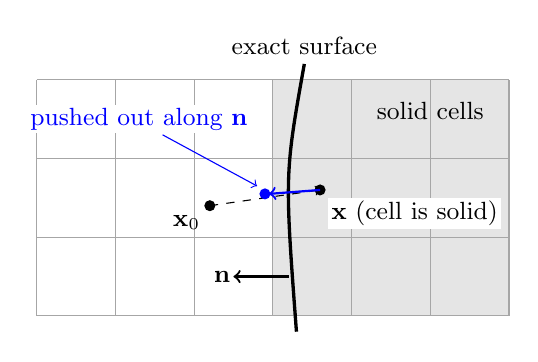
\begin{tikzpicture}[x=1cm,y=1cm,font=\small]
  \fill[black!10] (3,0) rectangle (6,3);
  \draw[step=1,black!35] (0,0) grid (6,3);
  \draw[very thick] (3.4,3.2) .. controls (3.15,1.8) .. (3.3,-0.2);
  \node[above] at (3.4,3.2) {exact surface};
  \node at (5,2.6) {solid cells};
  \fill (2.2,1.4) circle (2pt); \node[below left] at (2.2,1.4) {$\mathbf{x}_0$};
  \draw[->,dashed] (2.2,1.4) -- (3.6,1.6);
  \fill (3.6,1.6) circle (2pt); \node[below right,fill=white,inner sep=1pt] at (3.7,1.5) {$\mathbf{x}$ (cell is solid)};
  \fill[blue] (2.9,1.55) circle (2pt);
  \draw[->,thick,blue] (3.6,1.6) -- (2.95,1.55);
  \node[blue,fill=white,inner sep=1pt] at (1.3,2.5) {pushed out along $\mathbf{n}$}; \draw[blue,->] (1.6,2.3) -- (2.8,1.65);
  \draw[->,thick] (3.2,0.5) -- (2.5,0.5); \node[fill=white,inner sep=1pt,left] at (2.5,0.5) {$\mathbf{n}$};
\end{tikzpicture}
\end{center}

\subsection{Contact on gridless methods}\label{sec:contact-gridless}

SPH has no voxel mask, so \code{ResolveContactsAnalytic} uses the scene's exact surface alone and keeps a standoff
\code{margin} from every surface.
\begin{itemize}[itemsep=1pt,topsep=2pt]
\item A particle closer than \code{margin} to a face of the domain is put at that distance and gets the response with
  the wall's inward normal.
\item A particle inside a solid moves by $(-\phi + \text{margin})\,\mathbf{n}$ and gets the response with
  $\mathbf{n}$. On a medial axis it is left alone.
\item The order is walls, obstacles, walls, as on a grid.
\end{itemize}

% =====================================================================================================
\section{The Configuration file}\label{sec:config}

One config file describes a run. It holds \code{KEY = value} lines, then four kinds of block:
\code{PRESSURE_BEGIN} to \code{PRESSURE_END} for the shared pressure solver, one \code{<KEY>_BEGIN} to
\code{<KEY>_END} block per registered method, and \code{SCENE_BEGIN} to \code{SCENE_END} for the geometry
(Section~\ref{sec:scene-api}). A \texttt{\#} starts a comment, also after a value. A key that is left out takes the
default below. The setup screen writes every key, so a file it saves lists them all.

\textbf{Validation.} \code{InitializeSimulation} reads the whole file before it builds anything and stops the program
with exit code 1, listing every problem at once, when
\begin{itemize}[nosep]
  \item the file does not exist (\code{configuration file '...' not found});
  \item a key is not read by anything: a misspelling at the top level, or a key that is not in the table of the
    method block it sits in;
  \item a number does not parse in full (\code{VISCOSITY = abc} or \code{0.01abc}), or an integer key holds a real
    (\code{GRID_SIZE = 32.5});
  \item a choice is outside its list (\code{PROJECTION_SCHEME = FOO}), with the allowed values printed;
  \item a \code{REFINE_*} interval does not parse or is empty;
  \item a \code{<KEY>_BEGIN} block belongs to a method the program did not register.
\end{itemize}
The pressure block is checked by its backend (AMGX parses its own keys), and the scene block by the scene parser
(Section~\ref{sec:scene-api}). The setup screen opens the same file without stopping: it keeps the default for a
value it cannot read, and writes every key back, valid, when the case is saved.

\subsection{The run}

\begin{ktab}{\linewidth}{@{}>{\raggedright}p{0.30\linewidth} >{\raggedright}p{0.14\linewidth} X@{}}
\toprule
\textbf{Key} & \textbf{Default} & \textbf{Meaning} \\
\midrule
\code{DIMENSION} & 3 & 2 or 3. \\
\midrule
\code{TYPE} & the first method registered & the key of the method to run, for example \code{ADI}, \code{FLIP},
  \code{SPH} or \code{EXPLICIT}. A key that names no registered method stops the run with an error. \\
\midrule
\code{THREAD_COUNT} & 4 & OpenMP threads. \\
\midrule
\code{GPU_ACCELERATION} & 0 & 1 solves the pressure with AMGX. Forced to 0 in a build without the GPU. \\
\bottomrule
\end{ktab}

\subsection{Domain and grid}

\begin{ktab}{\linewidth}{@{}>{\raggedright}p{0.30\linewidth} >{\raggedright}p{0.14\linewidth} X@{}}
\toprule
\textbf{Key} & \textbf{Default} & \textbf{Meaning} \\
\midrule
\code{DOMAIN_X0}, \code{DOMAIN_XF}, \code{DOMAIN_Y0}, \code{DOMAIN_YF}, \code{DOMAIN_Z0}, \code{DOMAIN_ZF} & 0 &
  the extents of the domain, in metres. Always set them. \\
\midrule
\code{GRID_SIZE} & 16 & cells inside the domain across the shorter of the x and y lengths. The spacing is that length
  divided by \code{GRID_SIZE}, the same on every axis; the ring adds one cell outside each face. \\
\midrule
\code{NON_UNIFORM_GRID} & 0 & 1 enables the refinement below. Only a method with \code{CAP_RECTILINEAR} honours it;
  any other is given a uniform grid, with a warning. \\
\midrule
\code{REFINE_X}, \code{REFINE_Y}, \code{REFINE_Z} & none & refined intervals, separated by \code{;}, each
  \code{start end factor [mode]}. Mode \code{hard} (default) splits each cell into \code{factor} cells;
  \code{ramp} grows the factor from 1 at \code{start} to \code{factor} at \code{end}; \code{ramp_back} is its mirror;
  \code{graded} is 1 at both ends and \code{factor} in the middle. Where intervals overlap the finest wins.
  An interval outside the domain refines nothing. Section~\ref{sec:mac-construction} gives the construction. \\
\bottomrule
\end{ktab}
\begin{lstlisting}[style=ex]
NON_UNIFORM_GRID = 1
REFINE_X = 0 0.1 4 ramp ; 0.1 0.3 4 hard ; 0.3 0.7 4 ramp_back
\end{lstlisting}

\subsection{Fluid and reference values}

\begin{ktab}{\linewidth}{@{}>{\raggedright}p{0.30\linewidth} >{\raggedright}p{0.14\linewidth} X@{}}
\toprule
\textbf{Key} & \textbf{Default} & \textbf{Meaning} \\
\midrule
\code{VISCOSITY} & 0.01 & kinematic viscosity $\nu$, in m$^2$/s. \\
\midrule
\code{DENSITY} & 1 & density $\rho$, in kg/m$^3$. \\
\midrule
\code{Fu}, \code{Fv}, \code{Fw} & 0 & a uniform body force, as an acceleration in m/s$^2$ (gravity is
  \code{Fv = -9.81}). A force that varies in space or time is the scene's \code{force} directive. \\
\midrule
\code{MEAN_VELOCITY} & 1 & the reference speed $U$ of the force coefficients. \\
\midrule
\code{CHARACTERISTIC_LENGTH} & 0.1 & the reference length $L$ of the force coefficients. \\
\midrule
\code{CHARACTERISTIC_LENGTH_2} & the value of $L$ & in 3D the coefficients divide by the area
  $L \cdot L_2$ (diameter times span, chord times span). \\
\midrule
\code{REYNOLDS_NUMBER} & 0 & used only in the name of the output folder. The flow's Reynolds number follows from
  \code{VISCOSITY}, \code{MEAN_VELOCITY} and \code{CHARACTERISTIC_LENGTH}. \\
\bottomrule
\end{ktab}

\subsection{Time stepping and the end of the run}

\begin{ktab}{\linewidth}{@{}>{\raggedright}p{0.30\linewidth} >{\raggedright}p{0.14\linewidth} X@{}}
\toprule
\textbf{Key} & \textbf{Default} & \textbf{Meaning} \\
\midrule
\code{TIME_STEP} & 0 & the time step $\Delta t$, in seconds. Always set it. Under \code{ADAPTATIVE_TIMESTEP} it is
  the largest step allowed. \\
\midrule
\code{ADAPTATIVE_TIMESTEP} & 0 & 1 sets $\Delta t$ every step from \code{MAX_CFL}, or from the method's own stable
  step when its row gives one. \\
\midrule
\code{MAX_CFL} & 1 & the target advective CFL number $\Delta t\,|u|_{\max}/h$. \\
\midrule
\code{STOP_CONDITION} & \code{NEVER} & \code{NEVER}, \code{TIME} or \code{RESIDUAL}. A run without a window refuses
  \code{NEVER}. \\
\midrule
\code{STOP_TIME} & 1 & under \code{TIME}: the run ends exactly at this time, in seconds; the last step is shortened
  to land on it. \\
\midrule
\code{STOP_RESIDUAL} & $10^{-6}$ & under \code{RESIDUAL}: the run ends when the step residual (Section~\ref{sec:telemetry})
  falls below this. \\
\midrule
\code{STOP_EXPORT} & 1 & 1 writes the final field and telemetry row when the rule fires. \\
\bottomrule
\end{ktab}

\subsection{Output}

\begin{ktab}{\linewidth}{@{}>{\raggedright}p{0.36\linewidth} >{\raggedright}p{0.12\linewidth} X@{}}
\toprule
\textbf{Key} & \textbf{Default} & \textbf{Meaning} \\
\midrule
\code{EXPORT_ENABLED} & 1 & 0 writes nothing. \\
\midrule
\code{EXPORT_BASE_PATH} & \code{Exports} & the folder the run's folder is made in. \\
\midrule
\code{EXPORT_TELEMETRY_INTERVAL} & 1 & a telemetry row every this many steps. \\
\midrule
\code{EXPORT_FRAME_MODE} & \code{ITERATIONS} & when frames are written: every \code{EXPORT_GRID_INTERVAL} steps, or
  under \code{TIME} every \code{EXPORT_FRAME_INTERVAL} seconds of simulated time. \\
\midrule
\code{EXPORT_GRID_INTERVAL} & 100 & steps between frames. \\
\midrule
\code{EXPORT_FRAME_INTERVAL} & 0.04 & seconds between frames. \\
\midrule
\code{EXPORT_GRID} & 0 & 1 writes the field as \code{VTK/*.vtr}: velocity, pressure, cell type and the scalars. \\
\midrule
\code{EXPORT_PARTICLES} & 0 & 1 writes the particles as CSV (particle methods). \\
\midrule
\code{EXPORT_SURFACE} & 0 & 1 writes the liquid surface as PLY (3D particle methods). \\
\midrule
\code{EXPORT_SURFACE_SOLIDS} & 1 & with \code{EXPORT_SURFACE}: also the obstacles, once, as their own PLY. \\
\midrule
\code{EXPORT_SURFACE_VOXEL_SCALE}, \code{_RADIUS_SCALE}, \code{_INFLUENCE_SCALE} & 0.75, 1, 2 & the surface's
  lattice pitch, particle radius and averaging radius, in particle spacings. A larger influence radius gives a
  smoother surface. \\
\midrule
\code{EXPORT_SURFACE_SMOOTHING} & 2 & smoothing passes over the surface's distance field. \\
\midrule
\code{EXPORT_VOLUMETRIC} & 0 & 1 writes each scalar as a NumPy array per frame, with a JSON file of the grid. \\
\midrule
\code{EXPORT_AERODYNAMICS} & 0 & 1 computes and writes the force coefficients. \\
\midrule
\code{EXPORT_DAMBREAK} & 0 & 1 computes and writes the free-surface height and front. \\
\midrule
\code{EXPORT_COLUMN_*} & 1 & one flag per group of telemetry columns (Section~\ref{sec:telemetry}). \\
\bottomrule
\end{ktab}

\subsection{The pressure block}

The block configures the shared pressure solver (Section~\ref{sec:pressure-api}). It is written in every file and
read only by a method that uses that solver.
\begin{lstlisting}[style=ex]
PRESSURE_BEGIN
NEEDS_COMPATIBILITY_CONDITION = 1   # a pressure fixed only up to a constant (no pressure outlet)
PRESSURE_WARM_START = 0
eigen_solver = AMG                  # CPU: AMG (AMGCL), CG or BICGSTAB
eigen_tolerance = 1e-06
config_version=2                    # everything else is AMGX's own configuration (GPU)
solver=PCG
tolerance=1e-06
...
PRESSURE_END
\end{lstlisting}
\begin{ktab}{\linewidth}{@{}>{\raggedright}p{0.36\linewidth} >{\raggedright}p{0.14\linewidth} X@{}}
\toprule
\textbf{Key} & \textbf{Default} & \textbf{Meaning} \\
\midrule
\code{NEEDS_COMPATIBILITY_CONDITION} & 0 & 1 makes a singular system solvable: when no face fixes the pressure
  (every boundary a wall, an inlet or an outflow) the right-hand side's mean is removed. Required in that case. \\
\midrule
\code{PRESSURE_WARM_START} & 0 & 1 starts each Chorin solve from the previous pressure. \\
\midrule
\code{eigen_solver} & \code{BICGSTAB} & the CPU solver: \code{AMG} (CG with AMGCL's algebraic multigrid, the fastest),
  \code{CG} or \code{BICGSTAB}. \\
\midrule
\code{eigen_preconditioner} & \code{DIAGONAL} & for \code{CG} and \code{BICGSTAB}: \code{DIAGONAL}, \code{IDENTITY},
  \code{ILUT} or \code{IC}. \\
\midrule
\code{eigen_tolerance} & $10^{-9}$ (2D), $10^{-12}$ (3D) & the relative residual the CPU solve stops at. \\
\midrule
\code{eigen_max_iters} & 2000 & the CPU solve's iteration cap. \\
\midrule
any other line & & passed to AMGX as its configuration, see the AMGX reference. On a singular system set
  \code{amg_solver:coarse_solver=NOSOLVER}; AMGX's default dense coarse solve fails on it. \\
\bottomrule
\end{ktab}

\subsection{Particle options}

Read by every method with particles.
\begin{ktab}{\linewidth}{@{}>{\raggedright}p{0.30\linewidth} >{\raggedright}p{0.14\linewidth} X@{}}
\toprule
\textbf{Key} & \textbf{Default} & \textbf{Meaning} \\
\midrule
\code{PARTICLE_CONTACT} & \code{SLIP} & the contact response, \code{SLIP}, \code{NOSLIP} or \code{BOUNCE}
  (Section~\ref{sec:contact}). \\
\midrule
\code{PARTICLE_RESTITUTION} & 0.3 & the restitution $e$ under \code{BOUNCE}. \\
\midrule
\code{PARTICLE_SURFACE_OFFSET} & 0.01 & how far outside a surface a pushed-out particle is put, in cells. \\
\midrule
\code{PARTICLE_SEED_JITTER} & 0 & a random offset of each seeded particle, as a fraction of its spacing. \\
\bottomrule
\end{ktab}

\subsection{The method blocks}

Each method reads its own block, \code{ADI_BEGIN} to \code{ADI_END} and so on. The setup screen writes the blocks of
every registered method, so switching \code{TYPE} keeps the others' settings.

\begin{ktab}{\linewidth}{@{}>{\raggedright}p{0.32\linewidth} >{\raggedright}p{0.14\linewidth} X@{}}
\multicolumn{3}{@{}l}{\textbf{ADI}} \\[2pt]
\toprule
\textbf{Key} & \textbf{Default} & \textbf{Meaning} \\
\midrule
\code{CONVECTION_SCHEME} & \code{CENTRAL} & \code{CENTRAL} (second order) or \code{UPWIND} (first order, bounded). \\
\midrule
\code{CONVECTION_FORM} & \code{FLUX} & \code{FLUX} or \code{ADVECTIVE}. \\
\midrule
\code{PROJECTION_SCHEME} & \code{CHORIN} & \code{CHORIN} or \code{INCREMENTAL}. \\
\midrule
\code{VORTICITY_CONFINEMENT} & 0 & 1 adds a force that keeps small vortices from decaying. A graphics aid, not
  physics; no validated case uses it, and it will be removed in a future version. \\
\midrule
\code{VORTICITY_EPSILON} & 10 & its strength, in 1/s. \\
\midrule
\code{VORTICITY_SOLID_MARGIN} & 2 & no confinement within this many cells of a solid. \\
\bottomrule
\end{ktab}

\begin{ktab}{\linewidth}{@{}>{\raggedright}p{0.32\linewidth} >{\raggedright}p{0.14\linewidth} X@{}}
\multicolumn{3}{@{}l}{\textbf{FLIP}} \\[2pt]
\toprule
\textbf{Key} & \textbf{Default} & \textbf{Meaning} \\
\midrule
\code{PARTICLES_PER_CELL} & 4 & particles seeded per cell, 1 to 27. \\
\midrule
\code{ALPHA} & 1 & the blend of the particle update: 1 is FLIP, 0 is PIC. \\
\midrule
\code{PHYSICAL_DIFFUSION} & 0 & 1 solves the viscous term. \\
\midrule
\code{DIFFUSION_SOLVER} & \code{IMPLICIT} & \code{IMPLICIT} (one solve) or \code{ADI} (split by direction, cheaper). \\
\midrule
\code{FLIP_VISCOUS_PRESSURE} & 0 & 1 puts the body force and the old pressure gradient inside the viscous solve,
  for very viscous liquids. \\
\midrule
\code{FLIP_DENSITY_CORRECTION} & 0 & 1 moves the particles toward the rest density every step, which stops the
  liquid's volume from drifting. \\
\midrule
\code{FLIP_DENSITY_SURFACE_CLAMP} & 1 & with the correction: surface cells are not pulled inward. \\
\bottomrule
\end{ktab}

\begin{ktab}{\linewidth}{@{}>{\raggedright}p{0.32\linewidth} >{\raggedright}p{0.14\linewidth} X@{}}
\multicolumn{3}{@{}l}{\textbf{SPH}} \\[2pt]
\toprule
\textbf{Key} & \textbf{Default} & \textbf{Meaning} \\
\midrule
\code{SPH_KERNEL_RADIUS} & 0.05 & the kernel support radius, in metres: the method's resolution. \\
\midrule
\code{SPH_PARTICLE_SPACING} & 0 & the seeding pitch, in metres; 0 means the kernel radius over 2.6. \\
\midrule
\code{SPH_SOUND_SPEED} & 20 & the sound speed $c_0$, in m/s, at least ten times the fastest flow. \\
\midrule
\code{SPH_DELTA} & 0.1 & the density diffusion coefficient. \\
\midrule
\code{SPH_ALPHA} & 0.02 & the artificial viscosity. \\
\bottomrule
\end{ktab}

\begin{ktab}{\linewidth}{@{}>{\raggedright}p{0.32\linewidth} >{\raggedright}p{0.14\linewidth} X@{}}
\multicolumn{3}{@{}l}{\textbf{EXPLICIT}} \\[2pt]
\toprule
\textbf{Key} & \textbf{Default} & \textbf{Meaning} \\
\midrule
\code{EXPLICIT_RELAXATION} & 1.7 & the SOR factor $\omega$, 0.5 to 2. \\
\midrule
\code{EXPLICIT_TOLERANCE} & $10^{-6}$ & the largest residual, relative to the largest right-hand side. \\
\midrule
\code{EXPLICIT_MAX_ITERATIONS} & 10000 & the sweep cap. \\
\bottomrule
\end{ktab}

% =====================================================================================================
\section{The scene}\label{sec:scene-api}

The scene is a small language with one directive per line. A value is a number or an expression in
\code{x y z t dh Lx Ly Lz}. In an expression a leading minus sign binds tighter than \code{^}, so write a Gaussian as
\code{exp(0-(...)^2)}.

\begin{lstlisting}[style=ex]
boundary xmin inlet u="1.5*4*y*(0.41-y)/0.41^2" v="0"
boundary xmax pressure_outlet
boundary ymin noslip
boundary ymax noslip
region solid cylinder axis=z center=(0.2,0.2) radius=0.05
scalar smoke scheme=upwind form=flux
probe p_front p at=(0.15,0.2,0)
\end{lstlisting}

\begin{ktab}{\linewidth}{>{\ttfamily}p{0.27\linewidth} X}
\toprule
\normalfont\textbf{Directive} & \textbf{Meaning} \\
\midrule
boundary <face> <kind> & \code{face} is one of \code{xmin} to \code{zmax}. \code{kind} is \code{noslip},
  \code{slip}, \code{moving}, \code{inlet}, \code{pressure_outlet} or \code{outflow} (Section~\ref{sec:mac-bc}). A
  \code{moving} wall takes a tangential speed. An \code{inlet} takes its velocity, and \code{p=} sets the pressure
  level when the system has no other. A \code{pressure_outlet} takes \code{p=}, or 0 without it. Scalars take their
  values here, for example \code{smoke="1"}. A face that is not named is a no-slip wall. \\
\midrule
region <solid|fluid> <shape> & The shapes are \code{box min= max=}, \code{sphere center= radius=},
  \code{cylinder axis= center= radius=}, \code{plane point= normal=}, \code{mesh file= center= rotate= scale=} (a
  closed STL) and \code{naca00XX center= chord= pivot= rotate= [span=]}. \code{invert} keeps the outside. A
  \code{fluid} region is where a particle method seeds its liquid. \\
\midrule
scalar <name> & \code{solver=adi|none} (default \code{adi}), \code{scheme=central|upwind},
  \code{form=flux|advective}, \code{epsilon=}, \code{gamma=} and \code{source="..."}. With \code{solver=none} the
  field is held and its boundary set; \code{scheme} and \code{form} do not apply, and \code{epsilon}, \code{gamma}
  and \code{source} are kept for the method that updates it. It must come before any boundary that names
  it. \\
\midrule
force & \code{u= v= w=}. A body force, as an acceleration, added to the config's \code{Fu}, \code{Fv} and
  \code{Fw}. \\
\midrule
initial & \code{u= v= w=}. The velocity at time 0. \\
\midrule
probe <name> <quantity> & \code{at=(x,y,z)} and an optional \code{radius=}. Each probe adds one telemetry column
  (Section~\ref{sec:probes}). \\
\bottomrule
\end{ktab}

The parser is \code{src/headers/Core/Scene.h}. \code{ConfigReader} loads the block into the global \code{SCENE} and
binds the grid's boundary functions and cell types to it, so no solver reads the scene text. Within a list the later
line wins: a boundary declared last owns the edges and corners it shares, and a \code{fluid} region after a
\code{solid} one carves a hole in it.

\subsection{Probes}\label{sec:probes}

A probe writes one value per telemetry row, in a column named after the probe and its quantity, for example
\code{S1_p}. The value is the raw one, read from the field the step just produced. Any filtering or post-processing
is done afterwards, on the CSV.
\begin{lstlisting}[style=ex]
probe S1    p     at=(1.61,0.003,0.075) radius=0.0021   # a wall pressure sensor
probe H1    level at=(1.31,0,0.075)                     # a wave gauge
probe jet   top   at=(0.8,0,0)                          # the highest liquid, spray included
probe smoke smoke at=(0.5,0.2,0)                        # a declared scalar
\end{lstlisting}
The quantity is \code{p}, \code{u}, \code{v}, \code{w}, \code{speed}, \code{level}, \code{top} or the name of a
declared scalar. In 2D the third coordinate may be left out.

\textbf{Pressure and scalars.} Bilinear (2D) or trilinear (3D) interpolation between the cell centres $c$ around the
point, with weights $w_c$, solid cells left out and the rest renormalised,
\begin{equation*}
  P = \frac{\sum_{c\ \text{not solid}} w_c\,p_c}{\sum_{c\ \text{not solid}} w_c} .
\end{equation*}
A probe on a wall therefore reads the fluid beside it.

\textbf{Velocity.} \code{u}, \code{v} and \code{w} are interpolated on the staggered faces, and are 0 in a solid cell.
\code{speed} is the magnitude of the three.

\textbf{Radius.} With a radius $R$, every quantity except \code{level} and \code{top} becomes the volume-weighted
average over the cells $c$ whose centre lies within $R$ of the probe and that are not solid,
\begin{equation*}
  P = \frac{\sum_{c\,\in\,S} V_c\,P_c}{\sum_{c\,\in\,S} V_c}, \qquad
  S = \bigl\{\, c \;:\; |\mathbf{x}_c - \mathbf{x}_{\mathrm{probe}}| \le R,\ c \text{ not solid} \,\bigr\},
\end{equation*}
which models a sensor that reports the load over its face. When no centre lies within $R$ the probe falls back to the
point value.

\textbf{Level.} A wave gauge: the height of the liquid column connected to the bed. Each grid column is walked up from
the bottom, stepping over solid cells below the liquid, and its height $h_j$ is the top face of the last fluid cell
before the first cell that is not fluid. The probe's column is used, or with a radius every column whose centre is
within $R$, averaged by their cross-sections $A_j$,
\begin{equation*}
  H = \frac{\sum_j A_j\,h_j}{\sum_j A_j}.
\end{equation*}

\textbf{Top.} The largest $y$ among the particles within $R$ of the probe's vertical line (half a cell when $R$ is 0),
spray included. Without particles, the top face of the highest fluid cell in the column.

\begin{lstlisting}[style=sig]
struct Probe { std::string name, quantity; ProbeQuantity kind; double at[3]; double radius; };
\end{lstlisting}
One probe as the scene declared it. \code{SCENE.probes} holds them in declaration order.

\begin{lstlisting}[style=sig]
double EvaluateProbe(MAC *grid, const ParticleSet *particles, const Probe &probe);
\end{lstlisting}
Reads one probe. The telemetry calls it on \code{GRID_SOL} after each step. It does not change the grid.
\begin{params}
\p{grid}{the grid to read.}
\p{particles}{the particle set, for \code{top}. It may be empty.}
\p{probe}{the probe.}
\end{params}
\returns{the probe's value, in the units of its quantity.}
\example
\begin{lstlisting}[style=ex]
for (const Probe &pr : SCENE.probes)
    std::printf("%s_%s = %g\n", pr.name.c_str(), pr.quantity.c_str(),
                EvaluateProbe(SIMULATION.GRID_SOL, &SIMULATION.particles, pr));
\end{lstlisting}

% =====================================================================================================
\section{Telemetry}\label{sec:telemetry}

With \code{EXPORT_ENABLED = 1} the run writes \code{telemetry.csv} in its output folder: a header, then one row every
\code{EXPORT_TELEMETRY_INTERVAL} steps and one at the end of the run. Every value is read from the field the step
has just produced. A group of columns is left out when its \code{EXPORT_COLUMN_*} flag is 0 or, for the last three
groups, when its export flag is off. The columns appear in the order of the table.

\begin{ktab}{\linewidth}{@{}>{\raggedright}p{0.24\linewidth} >{\raggedright}p{0.22\linewidth} X@{}}
\toprule
\textbf{Column} & \textbf{Flag} & \textbf{Value} \\
\midrule
\code{iteration} & always & the number of steps completed. \\
\midrule
\code{time} & \code{_TIME} & the simulated time of the field, in seconds. \\
\midrule
\code{div_sum} & \code{_DIVERGENCE} & $\sum_c |(\nabla\cdot\mathbf u)_c|$ over the cells inside the domain, in 1/s;
  how well the projection made the field divergence free. \\
\midrule
\code{advcfl}, \code{diffcfl}, \code{cell_reynolds} & \code{_CFL} & $\Delta t\,|u|_{\max}/h$ and
  $\nu\,\Delta t/h^2$ with $h$ the smallest cell; the largest $|u_d|\,h_d/\nu$ over the faces, $h_d$ the spacing
  along the face's own axis. \\
\midrule
\code{residual} & \code{_RESIDUAL} & $\max |\mathbf u^{n+1} - \mathbf u^{n}|$ over every face: how far the flow
  still moves per step. \code{STOP_RESIDUAL} tests it. \\
\midrule
\code{<step>_timing} & \code{_STEP_TIMINGS} & one column per registered step: its wall time, in seconds. \\
\midrule
\code{<step>_counter} & \code{_STEP_TIMINGS} & one column per step: its work count, $-1$ for a step that reports
  none. \code{pressure_counter} is the pressure solve's iterations. \\
\midrule
\code{kinetic_energy}, \code{enstrophy}, \code{dE_dt} & \code{_FLOW_INTEGRALS} & volume averages per unit mass over
  the fluid: $E = \frac{1}{V}\int\frac{1}{2}|\mathbf u|^2\,dV$, $Z = \frac{1}{V}\int\frac{1}{2}|\boldsymbol\omega|^2
  \,dV$, and the backward difference of $E$ between rows (\code{nan} on the first). \\
\midrule
\code{cl}, \code{cd}, \code{cd_cv}, \code{cl_cv}, \code{ld_ratio} & \code{EXPORT_AERODYNAMICS} with \code{_CL},
  \code{_CD}, \code{_LD_RATIO} & the force coefficients of the solids inside the domain (below). \\
\midrule
\code{FluidHeight}, \code{FluidFront}, \code{FluidVolume} & \code{EXPORT_DAMBREAK} with \code{_FLUID_HEIGHT},
  \code{_FLUID_FRONT} & the free surface (below). \\
\midrule
\code{<name>_<quantity>} & always & one column per probe of the scene (Section~\ref{sec:probes}). \\
\bottomrule
\end{ktab}

\textbf{Force coefficients.} $F_x$ (drag) and $F_y$ (lift) are the force of the fluid on every solid inside the
domain, per unit span in 2D. The coefficients are
\begin{equation*}
  C_d = \frac{2F_x}{\rho\,U^2 S}, \qquad C_l = \frac{2F_y}{\rho\,U^2 S}, \qquad
  S = \begin{cases} L & \text{2D}, \\ L\,L_2 & \text{3D}, \end{cases}
\end{equation*}
with $U$ = \code{MEAN_VELOCITY}, $L$ = \code{CHARACTERISTIC_LENGTH} and $L_2$ = \code{CHARACTERISTIC_LENGTH_2}.
\code{cd} and \code{cl} integrate the stress over the staircase faces of the solid. \code{cd_cv} and \code{cl_cv}
take the momentum balance over a box around the body,
\begin{equation*}
  \mathbf F = \oint_{\partial B}\bigl(\boldsymbol\sigma\cdot\mathbf n - \rho\,\mathbf u\,(\mathbf u\cdot\mathbf n)\bigr)
  \,dS - \frac{d}{dt}\int_B \rho\,\mathbf u\,dV ,
\end{equation*}
with the box half the body's size beyond it on every side. The balance never touches the staircase, so it converges
where the surface integral does not; prefer it on a curved body. \code{ld_ratio} is $C_l/C_d$.

\textbf{Free surface.} On the cell types of the field (in 3D, on the plane through the middle of z):
\code{FluidHeight} is the top face of the highest fluid cell, and \code{FluidFront} the right face of the fluid cell
furthest along x, both in metres. \code{FluidVolume} is the number of fluid cells times their volume (an area in
2D); it is written for a particle method with a grid, where it shows the liquid's volume drift.

% =====================================================================================================
\section{The user interface}\label{sec:ui-api}

\code{src/headers/Core/SimulationManagerUI.h} declares four functions. \code{src/UI/SimulationManagerUI.cpp} defines
them, and only the GUI program compiles it. The setup screen, the viewer and the window sit behind these four
functions. \code{main} calls them from its own loop. The manager draws nothing and knows nothing about them.

\begin{lstlisting}[style=sig]
bool InitializeUI(std::string &configFile);
\end{lstlisting}
Opens the window and runs the setup screen until the user presses Start or closes the window.
\begin{params}
\p{configFile}{set to the path of the config the user chose. It is the file the setup screen saved last.}
\end{params}
\returns{true when the user pressed Start, false when the window was closed.}

\begin{lstlisting}[style=sig]
bool UpdateUI();
\end{lstlisting}
Draws one frame of the viewer and handles the window's controls, which run, pause, step and restart the simulation.
Call it once after each \code{StepSimulation}.
\returns{false once the window is closed, or when Restart was pressed.}

\begin{lstlisting}[style=sig]
bool RestartUI(std::string &configFile);
\end{lstlisting}
After \code{UpdateUI} returned false and the run was disposed: when that was a restart, runs the setup screen again.
\begin{params}
\p{configFile}{set to the path of the config the user chose.}
\end{params}
\returns{true when the user pressed Start, false when the window is closing.}

\begin{lstlisting}[style=sig]
void DisposeUI();
\end{lstlisting}
Closes the window and releases the graphical libraries. It is safe to call after \code{InitializeUI} returned false.
\example
\begin{lstlisting}[style=ex]
std::string config;
if (!InitializeUI(config)) { DisposeUI(); return 0; }
do
{
    SimulationManager::InitializeSimulation(config);
    Exports::InitializeTelemetry();
    do SimulationManager::StepSimulation(); while (UpdateUI());
    SimulationManager::DisposeSimulation();
} while (RestartUI(config));
DisposeUI();
\end{lstlisting}

\end{document}
